\UseRawInputEncoding
%DIF LATEXDIFF DIFFERENCE FILE
%DIF DEL ./old/compiled_v012.tex   Sat Jan 13 18:47:34 2024
%DIF ADD ./compiled.tex            Sat Jan 13 18:51:29 2024

%%%%%%%%%%%%%%%%%%%%%%%%%%%%%%%%%%%%%%%%%%%%%%%%%%%%%%%%%%%%%%%%%%%%%%%%%%%%%%%%
%% SETTINGS
%%%%%%%%%%%%%%%%%%%%%%%%%%%%%%%%%%%%%%%%%%%%%%%%%%%%%%%%%%%%%%%%%%%%%%%%%%%%%%%%
%% Columns
\documentclass[final,3p,times,twocolumn]{elsarticle}
%% Use the options 1p,twocolumn; 3p; 3p,twocolumn; 5p; or 5p,twocolumn
%% for a journal layout:
%% \documentclass[final,1p,times]{elsarticle}
%% \documentclass[final,1p,times,twocolumn]{elsarticle}
%% \documentclass[final,3p,times]{elsarticle}
%% \documentclass[final,3p,times,twocolumn]{elsarticle}
%% \documentclass[final,5p,times]{elsarticle}
%% \documentclass[final,5p,times,twocolumn]{elsarticle}
%% \documentclass[preprint,review,12pt]{elsarticle}

%% Image width
\newlength{\imagewidth}
\newlength{\imagescale}
%% preamble
\usepackage[english]{babel}
\usepackage[table]{xcolor} % For coloring tables
\usepackage{booktabs} % For professional quality tables
\usepackage{colortbl} % For coloring cells in tables
\usepackage{amsmath, amssymb} % For mathematical symbols and environments
\usepackage{amsthm} % For theorem-like environments
\usepackage{lipsum} % just for sample text
\usepackage{natbib}
\usepackage{graphicx}
\usepackage{indentfirst}
\usepackage{bashful}
\usepackage[margin=10pt,font=small,labelfont=bf,labelsep=endash]{caption}
\usepackage{graphicx}
\usepackage{calc}
\usepackage[T1]{fontenc} % [REVISED]
\usepackage[utf8]{inputenc} % [REVISED]
\usepackage{hyperref}
\usepackage{accsupp}
%% Line numbers
\linespread{1.1}
% \linenumbers
% Tables
\usepackage[pass]{geometry}
\usepackage{pdflscape}
\usepackage{csvsimple}
\usepackage{xltabular}
\usepackage{booktabs}
\usepackage{siunitx}
\usepackage{makecell}
\sisetup{round-mode=figures,round-precision=3}
\renewcommand\theadfont{\bfseries}
\renewcommand\theadalign{c}
\newcolumntype{C}[1]{>{\centering\arraybackslash}m{#1}}
\renewcommand{\arraystretch}{1.5}
\definecolor{lightgray}{gray}{0.95}

%% Diff
\usepackage{xcolor}
% Define commands for highlighting
% diff
\usepackage[most]{tcolorbox} % for boxes with transparency
% Define colors with transparency (opacity value)
\definecolor{GreenBG}{rgb}{0,1,0}
\definecolor{RedBG}{rgb}{1,0,0}
% Define tcolorbox environments for highlighting
\newtcbox{\greenhighlight}[1][]{%
  on line,
  colframe=GreenBG,
  colback=GreenBG!50!white, % 50% transparent green
  boxrule=0pt,
  arc=0pt,
  boxsep=0pt,
  left=1pt,
  right=1pt,
  top=2pt,
  bottom=2pt,
  tcbox raise base
}
\newtcbox{\redhighlight}[1][]{%
  on line,
  colframe=RedBG,
  colback=RedBG!50!white, % 50% transparent red
  boxrule=0pt,
  arc=0pt,
  boxsep=0pt,
  left=1pt,
  right=1pt,
  top=2pt,
  bottom=2pt,
  tcbox raise base
}
\newcommand{\REDSTARTS}{\color{red}}
\newcommand{\REDENDS}{\color{black}}
\newcommand{\GREENSTARTS}{\color{green}}
\newcommand{\GREENENDS}{\color{black}}
%%%%%%%%%%%%%%%%%%%%%%%%%%%%%%%%%%%%%%%%%%%%%%%%%%%%%%%%%%%%%%%%%%%%%%%%%%%%%%%%
%% JOURNAL NAME
%%%%%%%%%%%%%%%%%%%%%%%%%%%%%%%%%%%%%%%%%%%%%%%%%%%%%%%%%%%%%%%%%%%%%%%%%%%%%%%%
\journal{Heliyon}
%%%%%%%%%%%%%%%%%%%%%%%%%%%%%%%%%%%%%%%%%%%%%%%%%%%%%%%%%%%%%%%%%%%%%%%%%%%%%%%%
%% DOCUMENT STARTS
%%%%%%%%%%%%%%%%%%%%%%%%%%%%%%%%%%%%%%%%%%%%%%%%%%%%%%%%%%%%%%%%%%%%%%%%%%%%%%%%
%DIF PREAMBLE EXTENSION ADDED BY LATEXDIFF
%DIF UNDERLINE PREAMBLE %DIF PREAMBLE
\RequirePackage[normalem]{ulem} %DIF PREAMBLE
\RequirePackage{color}\definecolor{RED}{rgb}{1,0,0}\definecolor{BLUE}{rgb}{0,0,1} %DIF PREAMBLE
\providecommand{\DIFaddtex}[1]{{\protect\color{blue}\uwave{#1}}} %DIF PREAMBLE
\providecommand{\DIFdeltex}[1]{{\protect\color{red}\sout{#1}}}                      %DIF PREAMBLE
%DIF SAFE PREAMBLE %DIF PREAMBLE
\providecommand{\DIFaddbegin}{} %DIF PREAMBLE
\providecommand{\DIFaddend}{} %DIF PREAMBLE
\providecommand{\DIFdelbegin}{} %DIF PREAMBLE
\providecommand{\DIFdelend}{} %DIF PREAMBLE
\providecommand{\DIFmodbegin}{} %DIF PREAMBLE
\providecommand{\DIFmodend}{} %DIF PREAMBLE
%DIF FLOATSAFE PREAMBLE %DIF PREAMBLE
\providecommand{\DIFaddFL}[1]{\DIFadd{#1}} %DIF PREAMBLE
\providecommand{\DIFdelFL}[1]{\DIFdel{#1}} %DIF PREAMBLE
\providecommand{\DIFaddbeginFL}{} %DIF PREAMBLE
\providecommand{\DIFaddendFL}{} %DIF PREAMBLE
\providecommand{\DIFdelbeginFL}{} %DIF PREAMBLE
\providecommand{\DIFdelendFL}{} %DIF PREAMBLE
%DIF HYPERREF PREAMBLE %DIF PREAMBLE
\providecommand{\DIFadd}[1]{\texorpdfstring{\DIFaddtex{#1}}{#1}} %DIF PREAMBLE
\providecommand{\DIFdel}[1]{\texorpdfstring{\DIFdeltex{#1}}{}} %DIF PREAMBLE
\newcommand{\DIFscaledelfig}{0.5}
%DIF HIGHLIGHTGRAPHICS PREAMBLE %DIF PREAMBLE
\RequirePackage{settobox} %DIF PREAMBLE
\RequirePackage{letltxmacro} %DIF PREAMBLE
\newsavebox{\DIFdelgraphicsbox} %DIF PREAMBLE
\newlength{\DIFdelgraphicswidth} %DIF PREAMBLE
\newlength{\DIFdelgraphicsheight} %DIF PREAMBLE
% store original definition of \includegraphics %DIF PREAMBLE
\LetLtxMacro{\DIFOincludegraphics}{\includegraphics} %DIF PREAMBLE
\newcommand{\DIFaddincludegraphics}[2][]{{\color{blue}\fbox{\DIFOincludegraphics[#1]{#2}}}} %DIF PREAMBLE
\newcommand{\DIFdelincludegraphics}[2][]{% %DIF PREAMBLE
\sbox{\DIFdelgraphicsbox}{\DIFOincludegraphics[#1]{#2}}% %DIF PREAMBLE
\settoboxwidth{\DIFdelgraphicswidth}{\DIFdelgraphicsbox} %DIF PREAMBLE
\settoboxtotalheight{\DIFdelgraphicsheight}{\DIFdelgraphicsbox} %DIF PREAMBLE
\scalebox{\DIFscaledelfig}{% %DIF PREAMBLE
\parbox[b]{\DIFdelgraphicswidth}{\usebox{\DIFdelgraphicsbox}\\[-\baselineskip] \rule{\DIFdelgraphicswidth}{0em}}\llap{\resizebox{\DIFdelgraphicswidth}{\DIFdelgraphicsheight}{% %DIF PREAMBLE
\setlength{\unitlength}{\DIFdelgraphicswidth}% %DIF PREAMBLE
\begin{picture}(1,1)% %DIF PREAMBLE
\thicklines\linethickness{2pt} %DIF PREAMBLE
{\color[rgb]{1,0,0}\put(0,0){\framebox(1,1){}}}% %DIF PREAMBLE
{\color[rgb]{1,0,0}\put(0,0){\line( 1,1){1}}}% %DIF PREAMBLE
{\color[rgb]{1,0,0}\put(0,1){\line(1,-1){1}}}% %DIF PREAMBLE
\end{picture}% %DIF PREAMBLE
}\hspace*{3pt}}} %DIF PREAMBLE
} %DIF PREAMBLE
\LetLtxMacro{\DIFOaddbegin}{\DIFaddbegin} %DIF PREAMBLE
\LetLtxMacro{\DIFOaddend}{\DIFaddend} %DIF PREAMBLE
\LetLtxMacro{\DIFOdelbegin}{\DIFdelbegin} %DIF PREAMBLE
\LetLtxMacro{\DIFOdelend}{\DIFdelend} %DIF PREAMBLE
\DeclareRobustCommand{\DIFaddbegin}{\DIFOaddbegin \let\includegraphics\DIFaddincludegraphics} %DIF PREAMBLE
\DeclareRobustCommand{\DIFaddend}{\DIFOaddend \let\includegraphics\DIFOincludegraphics} %DIF PREAMBLE
\DeclareRobustCommand{\DIFdelbegin}{\DIFOdelbegin \let\includegraphics\DIFdelincludegraphics} %DIF PREAMBLE
\DeclareRobustCommand{\DIFdelend}{\DIFOaddend \let\includegraphics\DIFOincludegraphics} %DIF PREAMBLE
\LetLtxMacro{\DIFOaddbeginFL}{\DIFaddbeginFL} %DIF PREAMBLE
\LetLtxMacro{\DIFOaddendFL}{\DIFaddendFL} %DIF PREAMBLE
\LetLtxMacro{\DIFOdelbeginFL}{\DIFdelbeginFL} %DIF PREAMBLE
\LetLtxMacro{\DIFOdelendFL}{\DIFdelendFL} %DIF PREAMBLE
\DeclareRobustCommand{\DIFaddbeginFL}{\DIFOaddbeginFL \let\includegraphics\DIFaddincludegraphics} %DIF PREAMBLE
\DeclareRobustCommand{\DIFaddendFL}{\DIFOaddendFL \let\includegraphics\DIFOincludegraphics} %DIF PREAMBLE
\DeclareRobustCommand{\DIFdelbeginFL}{\DIFOdelbeginFL \let\includegraphics\DIFdelincludegraphics} %DIF PREAMBLE
\DeclareRobustCommand{\DIFdelendFL}{\DIFOaddendFL \let\includegraphics\DIFOincludegraphics} %DIF PREAMBLE
%DIF LISTINGS PREAMBLE %DIF PREAMBLE
\RequirePackage{listings} %DIF PREAMBLE
\RequirePackage{color} %DIF PREAMBLE
\lstdefinelanguage{DIFcode}{ %DIF PREAMBLE
%DIF DIFCODE_UNDERLINE %DIF PREAMBLE
  moredelim=[il][\color{red}\sout]{\%DIF\ <\ }, %DIF PREAMBLE
  moredelim=[il][\color{blue}\uwave]{\%DIF\ >\ } %DIF PREAMBLE
} %DIF PREAMBLE
\lstdefinestyle{DIFverbatimstyle}{ %DIF PREAMBLE
	language=DIFcode, %DIF PREAMBLE
	basicstyle=\ttfamily, %DIF PREAMBLE
	columns=fullflexible, %DIF PREAMBLE
	keepspaces=true %DIF PREAMBLE
} %DIF PREAMBLE
\lstnewenvironment{DIFverbatim}{\lstset{style=DIFverbatimstyle}}{} %DIF PREAMBLE
\lstnewenvironment{DIFverbatim*}{\lstset{style=DIFverbatimstyle,showspaces=true}}{} %DIF PREAMBLE
%DIF END PREAMBLE EXTENSION ADDED BY LATEXDIFF

\begin{document}

%%%%%%%%%%%%%%%%%%%%%%%%%%%%%%%%%%%%%%%%%%%%%%%%%%%%%%%%%%%%%%%%%%%%%%%%%%%%%%%%
%% Frontmatter
%%%%%%%%%%%%%%%%%%%%%%%%%%%%%%%%%%%%%%%%%%%%%%%%%%%%%%%%%%%%%%%%%%%%%%%%%%%%%%%%
\begin{frontmatter}
\begin{highlights}
\pdfbookmark[1]{Highlights}{highlights}

\item Neural trajectories in the hippocampus exhibited greater variability during a working memory (WM) task compared to those in the entorhinal cortex and amygdala regions.

\item The distance of neural trajectories between encoding and retrieval states in the hippocampus was memory-load dependent during a WM task.


\item Hippocampal neural trajectories fluctuated between the encoding and retrieval states in a task-dependent manner during both baseline and sharp-wave ripple (SWR) periods.

\item Hippocampal neural trajectories shifted from encoding to retrieval states during SWR period.

\end{highlights}\title{
Hippocampal neural fluctuations between memory encoding and retrieval states during a working memory task in humans
}\author[1]{Yusuke Watanabe\corref{cor1}}
\author[2,3,4]{Yuji Ikegaya}
\author[1,5]{Takufumi Yanagisawa}

\address[1]{Institute for Advanced Cocreation studies, Osaka University, 2-2 Yamadaoka, Suita, 565-0871, Osaka, Japan}
\address[2]{Graduate School of Pharmaceutical Sciences, The University of Tokyo, 7-3-1 Hongo, Tokyo, 113-0033, Japan}
\address[3]{Institute for AI and Beyond, The University of Tokyo, 7-3-1 Hongo, Tokyo, 113-0033, Japan}
\address[4]{Center for Information and Neural Networks, National Institute of Information and Communications Technology, 1-4 Yamadaoka, Suita City, 565-0871, Osaka, Japan}
\address[5]{Department of Neurosurgery, Osaka University Graduate School of Medicine, 2-2 Yamadaoka, Osaka, 565-0871, Japan}

\cortext[cor1]{Corresponding author. Tel: +81-6-6879-3652}%%Graphical abstract
%\pdfbookmark[1]{Graphical Abstract}{graphicalabstract}        
%\begin{graphicalabstract}
%\includegraphics{grabs}
%\end{graphicalabstract}
\begin{abstract}
\pdfbookmark[1]{Abstract}{abstract}
Working memory (WM) \DIFdelbegin \DIFdel{is a vital component in numerous }\DIFdelend \DIFaddbegin \DIFadd{plays a critical role in many }\DIFaddend cognitive functions, \DIFdelbegin \DIFdel{yet the complex }\DIFdelend \DIFaddbegin \DIFadd{but the intricate }\DIFaddend neural mechanisms that \DIFdelbegin \DIFdel{sustain its operation are not fully understood. In particular}\DIFdelend \DIFaddbegin \DIFadd{support its operation remain elusive. Specifically}\DIFaddend , while the hippocampus and sharp-wave ripple complexes (SWRs) \DIFdelbegin \DIFdel{--- }\DIFdelend \DIFaddbegin \DIFadd{-- }\DIFaddend brief, synchronous neural oscillation observed in the hippocampus \DIFdelbegin \DIFdel{--- are known }\DIFdelend \DIFaddbegin \DIFadd{-- are recognized }\DIFaddend for their roles in memory consolidation and retrieval, their \DIFdelbegin \DIFdel{engagement }\DIFdelend \DIFaddbegin \DIFadd{involvement }\DIFaddend in WM tasks \DIFdelbegin \DIFdel{remains unclear. Our current research posits that the }\DIFdelend \DIFaddbegin \DIFadd{has not yet been defined. Current research suggests that during WM tasks, }\DIFaddend multiunit activity patterns in the hippocampus \DIFdelbegin \DIFdel{exhibit unique dynamism during WM tasks, especially }\DIFdelend \DIFaddbegin \DIFadd{display distinctive dynamics, particularly }\DIFaddend during SWR periods. \DIFdelbegin \DIFdel{Our study involved the analysis of a dataset obtained }\DIFdelend \DIFaddbegin \DIFadd{This study analyzed a dataset derived }\DIFaddend from intracranial electroencephalogram recordings \DIFdelbegin \DIFdel{recorded from }\DIFdelend \DIFaddbegin \DIFadd{made in }\DIFaddend the medial temporal lobe (MTL) of nine individuals with epilepsy \DIFdelbegin \DIFdel{performing }\DIFdelend \DIFaddbegin \DIFadd{during }\DIFaddend an eight-second Sternberg task. We \DIFdelbegin \DIFdel{utilized }\DIFdelend \DIFaddbegin \DIFadd{applied }\DIFaddend Gaussian-process factor analysis to \DIFdelbegin \DIFdel{calculate }\DIFdelend \DIFaddbegin \DIFadd{determine }\DIFaddend low-dimensional neural representations, or 'trajectories,' within the MTL regions \DIFdelbegin \DIFdel{during }\DIFdelend \DIFaddbegin \DIFadd{while performing }\DIFaddend the WM task. \DIFdelbegin \DIFdel{Our results revealed that the neural trajectories showed }\DIFdelend \DIFaddbegin \DIFadd{The results indicate }\DIFaddend significant variations in the hippocampus\DIFdelbegin \DIFdel{compared to }\DIFdelend \DIFaddbegin \DIFadd{' neural trajectories compared to those in }\DIFaddend the entorhinal cortex and amygdala. \DIFdelbegin \DIFdel{Furthermore, }\DIFdelend \DIFaddbegin \DIFadd{Additionally, the }\DIFaddend distance of the trajectory between \DIFaddbegin \DIFadd{the }\DIFaddend encoding and retrieval phases \DIFdelbegin \DIFdel{were memory-load dependent . Crucially}\DIFdelend \DIFaddbegin \DIFadd{was dependent on memory load. Importantly}\DIFaddend , hippocampal trajectories during the retrieval phase \DIFdelbegin \DIFdel{fluctuated }\DIFdelend \DIFaddbegin \DIFadd{demonstrated variations }\DIFaddend between encoding and retrieval stages \DIFdelbegin \DIFdel{in a task-type dependent manner; especially showing transitions }\DIFdelend \DIFaddbegin \DIFadd{based on task type, particularly showing shifts }\DIFaddend from encoding to retrieval states during SWRs. \DIFdelbegin \DIFdel{Therefore, these observations not only demonstrate }%DIFDELCMD < [%%%
\DIFdel{FIXME>}%DIFDELCMD < ]%%%
\DIFdel{the integral role of}%DIFDELCMD < [%%%
\DIFdel{<FIXME}%DIFDELCMD < ] %%%
\DIFdel{the hippocampusin }%DIFDELCMD < [%%%
\DIFdel{FIXME>}%DIFDELCMD < ]%%%
\DIFdel{executing}%DIFDELCMD < [%%%
\DIFdel{<FIXME}%DIFDELCMD < ] %%%
\DIFdel{WM tasks but also }%DIFDELCMD < [%%%
\DIFdel{FIXME>}%DIFDELCMD < ]%%%
\DIFdel{put forth a compelling hypothesis }%DIFDELCMD < [%%%
\DIFdel{<FIXME}%DIFDELCMD < ] %%%
\DIFdel{for further investigation: the }%DIFDELCMD < [%%%
\DIFdel{FIXME>}%DIFDELCMD < ]%%%
\DIFdel{operational}%DIFDELCMD < [%%%
\DIFdel{<FIXME}%DIFDELCMD < ] %%%
\DIFdelend \DIFaddbegin \DIFadd{These findings underline the hippocampus's essential function in performing WM tasks and propose an intriguing hypothesis for future research: the functional }\DIFaddend state of the hippocampus \DIFdelbegin \DIFdel{shifts }\DIFdelend \DIFaddbegin \DIFadd{transition }\DIFaddend from encoding to retrieval during SWRs.
\end{abstract}% \pdfbookmark[1]{Keywords}{keywords}                
\begin{keyword}
working memory \sep memory load \sep hippocampus \sep sharp-wave ripples \sep humans
\end{keyword}
\end{frontmatter}

%%%%%%%%%%%%%%%%%%%%%%%%%%%%%%%%%%%%%%%%%%%%%%%%%%%%%%%%%%%%%%%%%%%%%%%%%%%%%%%%
%% IMRaD
%%%%%%%%%%%%%%%%%%%%%%%%%%%%%%%%%%%%%%%%%%%%%%%%%%%%%%%%%%%%%%%%%%%%%%%%%%%%%%%%

%%%%%%%%%%%%%%%%%%%%%%%%%%%%%%%%%%%%%%%%%%%%%%%%%%%%%%%%%%%%%%%%%%%%%%%%%%%%%%%%
%% INTRODUCTION
%%%%%%%%%%%%%%%%%%%%%%%%%%%%%%%%%%%%%%%%%%%%%%%%%%%%%%%%%%%%%%%%%%%%%%%%%%%%%%%%
\section{Introduction}
Working memory (WM) \DIFdelbegin \DIFdel{plays a crucial role in }\DIFdelend \DIFaddbegin \DIFadd{significantly influences }\DIFaddend everyday life, and \DIFdelbegin \DIFdel{its neural underpinnings remain an area of ongoing research. The hippocampus, notably }\DIFdelend \DIFaddbegin \DIFadd{the neural bases of this cognitive process continue to be the subject of intensive research. One key focus of this research is the hippocampus, a structure }\DIFaddend integral to memory \DIFdelbegin \DIFdel{, continues to be a primary focus of this investigation }\DIFdelend \DIFaddbegin \DIFadd{functions }\DIFaddend \cite{scoville_loss_1957} \cite{squire_legacy_2009}  \cite{boran_persistent_2019} \cite{kaminski_persistently_2017} \cite{kornblith_persistent_2017} \cite{faraut_dataset_2018} \cite{borders_hippocampus_2022} \cite{li_functional_2023} \cite{dimakopoulos_information_2022}. \DIFdelbegin \DIFdel{Gaining insights into the role }\DIFdelend \DIFaddbegin \DIFadd{A thorough understanding }\DIFaddend of the hippocampus\DIFaddbegin \DIFadd{'s role }\DIFaddend in working memory is \DIFdelbegin \DIFdel{vital to deepening our understanding }\DIFdelend \DIFaddbegin \DIFadd{essential for advancing our knowledge }\DIFaddend of cognitive processes \DIFdelbegin \DIFdel{, }\DIFdelend [\DIFdelbegin \DIFdel{FIXME}\DIFdelend \DIFaddbegin \DIFadd{CHECKME}\DIFaddend >]\DIFdelbegin \DIFdel{potentially fostering the progression of }\DIFdelend \DIFaddbegin \DIFadd{and fostering advancements in }\DIFaddend cognitive training and interventions[<\DIFdelbegin \DIFdel{FIXME}\DIFdelend \DIFaddbegin \DIFadd{CHECKME ENDS}\DIFaddend ]\DIFaddbegin \DIFadd{.
}\DIFaddend \\
\indent
Current evidence suggests \DIFaddbegin \DIFadd{that }\DIFaddend a transient, synchronized oscillation, \DIFdelbegin \DIFdel{referred to as }\DIFdelend \DIFaddbegin \DIFadd{called }\DIFaddend sharp-wave ripple (SWR) \cite{buzsaki_hippocampal_2015}, is \DIFdelbegin \DIFdel{linked }\DIFdelend \DIFaddbegin \DIFadd{associated }\DIFaddend with several cognitive functions\DIFdelbegin \DIFdel{, such as }\DIFdelend \DIFaddbegin \DIFadd{. These include }\DIFaddend memory replay \cite{wilson_reactivation_1994} \cite{nadasdy_replay_1999} \cite{lee_memory_2002} \cite{diba_forward_2007} \cite{davidson_hippocampal_2009}, memory consolidation \cite{girardeau_selective_2009} \cite{ego-stengel_disruption_2010} \cite{fernandez-ruiz_long-duration_2019} \cite{kim_corticalhippocampal_2022}, memory recall \cite{wu_hippocampal_2017} \cite{norman_hippocampal_2019} \cite{norman_hippocampal_2021}, and neural plasticity \cite{behrens_induction_2005} \cite{norimoto_hippocampal_2018}. This \DIFdelbegin \DIFdel{evidence indicates the likelihood that SWR could be a critical component }\DIFdelend \DIFaddbegin \DIFadd{association suggests that SWR may be a crucial part }\DIFaddend of hippocampal processing \DIFdelbegin \DIFdel{, contributing }\DIFdelend \DIFaddbegin \DIFadd{that contributes }\DIFaddend to working memory performance. However, research \DIFdelbegin \DIFdel{investigating }\DIFdelend \DIFaddbegin \DIFadd{on }\DIFaddend the effects of SWRs on working memory \DIFdelbegin \DIFdel{remains sparse }\DIFdelend \DIFaddbegin \DIFadd{is relatively scarce }\DIFaddend \cite{jadhav_awake_2012}, and is \DIFdelbegin \DIFdel{largely }\DIFdelend \DIFaddbegin \DIFadd{predominantly }\DIFaddend limited to rodent models \DIFdelbegin \DIFdel{participating }\DIFdelend \DIFaddbegin \DIFadd{engaged }\DIFaddend in navigation tasks\DIFdelbegin \DIFdel{where the exact }\DIFdelend \DIFaddbegin \DIFadd{, where the }\DIFaddend timing of memory acquisition and recall is not \DIFdelbegin \DIFdel{explicitly distinguished}\DIFdelend \DIFaddbegin \DIFadd{clearly defined}\DIFaddend .
\\
\indent
Recent studies \DIFdelbegin \DIFdel{indicate that hippocampal neurons exhibit }\DIFdelend \DIFaddbegin \DIFadd{have found }\DIFaddend low-dimensional representations \DIFaddbegin \DIFadd{in the hippocampal neurons }\DIFaddend during WM tasks. \DIFdelbegin \DIFdel{Notably}\DIFdelend \DIFaddbegin \DIFadd{Specifically}\DIFaddend , the firing patterns of place cells \cite{okeefe_hippocampus_1971} \cite{okeefe_place_1976} \cite{ekstrom_cellular_2003} \cite{kjelstrup_finite_2008} \cite{harvey_intracellular_2009}, \DIFdelbegin \DIFdel{located }\DIFdelend \DIFaddbegin \DIFadd{found }\DIFaddend in the hippocampus, \DIFdelbegin \DIFdel{are observed to be encompassed }\DIFdelend \DIFaddbegin \DIFadd{have been identified }\DIFaddend within a dynamic, nonlinear three-dimensional hyperbolic \DIFdelbegin \DIFdel{geometry in rat \mbox{%DIFAUXCMD
\cite{zhang_hippocampal_2022}}\hspace{0pt}%DIFAUXCMD
. Moreover}\DIFdelend \DIFaddbegin \DIFadd{space in rats \mbox{%DIFAUXCMD
\cite{zhang_hippocampal_2022}}\hspace{0pt}%DIFAUXCMD
. Additionally}\DIFaddend , grid cells in the entorhinal cortex (EC)\DIFdelbegin \DIFdel{-- the dominant }\DIFdelend \DIFaddbegin \DIFadd{, which is the main }\DIFaddend pathway to the hippocampus \cite{naber_reciprocal_2001} \cite{van_strien_anatomy_2009} \cite{strange_functional_2014}\DIFdelbegin \DIFdel{-- displayed toroidal topology during exploration \mbox{%DIFAUXCMD
\cite{gardner_toroidal_2022} }\hspace{0pt}%DIFAUXCMD
in rat. Unfortunately, these investigations are confined to }\DIFdelend \DIFaddbegin \DIFadd{, exhibited a toroidal geometry during exploration in rats \mbox{%DIFAUXCMD
\cite{gardner_toroidal_2022}}\hspace{0pt}%DIFAUXCMD
. However, these studies are limited by their focus on }\DIFaddend spatial navigation tasks in rodents, \DIFdelbegin \DIFdel{thus imposing limitations on }\DIFdelend \DIFaddbegin \DIFadd{affecting }\DIFaddend the temporal resolution of WM tasks [\DIFdelbegin \DIFdel{FIXME}\DIFdelend \DIFaddbegin \DIFadd{CHECKME}\DIFaddend >]\DIFdelbegin \DIFdel{like when the animal acquire and recallinformation}\DIFdelend \DIFaddbegin \DIFadd{such as the timing of information acquisition and recall}\DIFaddend [<\DIFdelbegin \DIFdel{FIXME}\DIFdelend \DIFaddbegin \DIFadd{CHECKME ENDS}\DIFaddend ]. The \DIFdelbegin \DIFdel{generalizability }\DIFdelend \DIFaddbegin \DIFadd{applicability }\DIFaddend of these findings to human subjects and beyond navigation tasks \DIFdelbegin \DIFdel{remains to be established}\DIFdelend \DIFaddbegin \DIFadd{still needs to be confirmed}\DIFaddend .
\\
\indent
\DIFdelbegin \DIFdel{Given these considerations, the current }\DIFdelend \DIFaddbegin \DIFadd{Considering these aspects, the present }\DIFaddend study aims to \DIFdelbegin \DIFdel{validate }\DIFdelend \DIFaddbegin \DIFadd{investigate }\DIFaddend the hypothesis that hippocampal neurons \DIFdelbegin \DIFdel{exhibit distinctive , }%DIFDELCMD < [%%%
\DIFdel{FIXME>}%DIFDELCMD < ]%%%
\DIFdel{responsible}%DIFDELCMD < [%%%
\DIFdel{<FIXME}%DIFDELCMD < ] %%%
\DIFdel{representations }\DIFdelend \DIFaddbegin \DIFadd{display distinctive patterns of activity or 'neural trajectories' }\DIFaddend in low-dimensional spaces, \DIFdelbegin \DIFdel{designated as 'neural trajectory, ' }%DIFDELCMD < [%%%
\DIFdel{FIXME>}%DIFDELCMD < ]%%%
\DIFdel{responsible to }%DIFDELCMD < [%%%
\DIFdel{<FIXME}%DIFDELCMD < ] %%%
\DIFdel{WM tasks, especially within SWR periods. To evaluate this claim, we employed }\DIFdelend \DIFaddbegin \DIFadd{particularly during SWR periods, in response to WM tasks. To test this hypothesis, we used }\DIFaddend a dataset of patients performing an eight-second Sternberg task \DIFdelbegin \DIFdel{with high temporal resolution }\DIFdelend (1 s for fixation, 2 s for encoding, 3 s for maintenance, and 2 s for retrieval) \DIFdelbegin \DIFdel{, while their intracranial electroencephalography signals }\DIFdelend \DIFaddbegin \DIFadd{with high temporal resolution. Intracranial electroencephalography }\DIFaddend (iEEG) \DIFaddbegin \DIFadd{signals }\DIFaddend within the medial temporal lobe (MTL) were \DIFdelbegin \DIFdel{being recorded }\DIFdelend \DIFaddbegin \DIFadd{recorded for these patients }\DIFaddend \cite{boran_dataset_2020}. To \DIFdelbegin \DIFdel{investigate }\DIFdelend \DIFaddbegin \DIFadd{examine }\DIFaddend low-dimensional neural trajectories, we \DIFdelbegin \DIFdel{employed }\DIFdelend \DIFaddbegin \DIFadd{utilized }\DIFaddend Gaussian-process factor analysis (GPFA), \DIFdelbegin \DIFdel{a method renowned }\DIFdelend \DIFaddbegin \DIFadd{an established method }\DIFaddend for analyzing neural population dynamics \cite{yu_gaussian-process_2009}.
\label{sec:introduction}
%%%%%%%%%%%%%%%%%%%%%%%%%%%%%%%%%%%%%%%%%%%%%%%%%%%%%%%%%%%%%%%%%%%%%%%%%%%%%%%%
%% METHODS
%%%%%%%%%%%%%%%%%%%%%%%%%%%%%%%%%%%%%%%%%%%%%%%%%%%%%%%%%%%%%%%%%%%%%%%%%%%%%%%%
\section{Methods}
\subsection{Dataset}
\DIFdelbegin \DIFdel{A publicly available dataset \mbox{%DIFAUXCMD
\cite{boran_dataset_2020} }\hspace{0pt}%DIFAUXCMD
was used, which consists }\DIFdelend \DIFaddbegin \DIFadd{The dataset employed in this study was publicly available and consisted }\DIFaddend of nine epilepsy patients performing a modified Sternberg task \DIFaddbegin \DIFadd{\mbox{%DIFAUXCMD
\cite{boran_dataset_2020}}\hspace{0pt}%DIFAUXCMD
}\DIFaddend . This task \DIFdelbegin \DIFdel{involves }\DIFdelend \DIFaddbegin \DIFadd{encompassed }\DIFaddend four phases: fixation (1s), encoding (2s), maintenance (3s), and retrieval (2s)\DIFdelbegin \DIFdel{\mbox{%DIFAUXCMD
\cite{boran_dataset_2020}}\hspace{0pt}%DIFAUXCMD
}\DIFdelend . During the encoding phase, participants were \DIFdelbegin \DIFdel{exposed to }\DIFdelend \DIFaddbegin \DIFadd{presented with }\DIFaddend four, six, or eight alphabet letters, \DIFdelbegin \DIFdel{referred to }\DIFdelend \DIFaddbegin \DIFadd{defined }\DIFaddend as the set size. \DIFdelbegin \DIFdel{Subsequently, they }\DIFdelend \DIFaddbegin \DIFadd{They }\DIFaddend [FIXME>]\DIFdelbegin \DIFdel{had }\DIFdelend \DIFaddbegin \DIFadd{were required }\DIFaddend to[<FIXME] \DIFdelbegin \DIFdel{decide }\DIFdelend \DIFaddbegin \DIFadd{ascertain }\DIFaddend whether a probe letter \DIFdelbegin \DIFdel{presented }\DIFdelend \DIFaddbegin \DIFadd{shown }\DIFaddend during the retrieval phase \DIFdelbegin \DIFdel{was previously displayed }\DIFdelend \DIFaddbegin \DIFadd{had appeared before }\DIFaddend (the correct choice for the Match IN task) or not (the correct choice for the Mismatch OUT task). \DIFdelbegin \DIFdel{iEEG signals were recorded at a sampling rate of }\DIFdelend \DIFaddbegin \DIFadd{Intracranial electroencephalography (iEEG) signals were captured with a }\DIFaddend 32 kHz \DIFdelbegin \DIFdel{, within a frequency range of }\DIFdelend \DIFaddbegin \DIFadd{sampling rate within a }\DIFaddend 0.5--5,000 Hz \DIFaddbegin \DIFadd{frequency range}\DIFaddend , using depth electrodes \DIFdelbegin \DIFdel{implanted in the }\DIFdelend \DIFaddbegin \DIFadd{in }\DIFaddend medial temporal lobe (MTL) regions: the anterior head of the left and \DIFdelbegin \DIFdel{the }\DIFdelend right hippocampus (AHL and AHR), the posterior body of the hippocampus (PHL and PHR), the entorhinal cortex (ECL and ECR), and the amygdala (AL and AR), as \DIFdelbegin \DIFdel{illustrated }\DIFdelend \DIFaddbegin \DIFadd{depicted }\DIFaddend in Figure~\ref{fig:01}A and Table~\ref{tab:01}. The iEEG signals were subsequently downsampled to \DIFdelbegin \DIFdel{a rate of }\DIFdelend 2 kHz. Correlations \DIFdelbegin \DIFdel{among }\DIFdelend \DIFaddbegin \DIFadd{between }\DIFaddend variables such as set size and correct rate were \DIFdelbegin \DIFdel{investigated }\DIFdelend \DIFaddbegin \DIFadd{examined }\DIFaddend (Figure~\ref{fig:s01}S1). \DIFdelbegin \DIFdel{The timings of multiunit spikes were determined by }\DIFdelend \DIFaddbegin \DIFadd{Multiunit spike timings were determined via }\DIFaddend a spike sorting algorithm \cite{niediek_reliable_2016} using the Combinato package (\url{https://github.com/jniediek/combinato})(Figure~\ref{fig:01}C).

\subsection{Calculation of neural trajectories using GPFA}
Neural trajectories, also \DIFdelbegin \DIFdel{termed }\DIFdelend \DIFaddbegin \DIFadd{referred to as }\DIFaddend 'factors' (Figure~\ref{fig:01}D), in the hippocampus, EC, and amygdala \DIFdelbegin \DIFdel{(Figure~\ref{fig:01}D), were computed }\DIFdelend \DIFaddbegin \DIFadd{were determined }\DIFaddend using GPFA \cite{yu_gaussian-process_2009} applied to the multiunit activity data for each session\DIFdelbegin \DIFdel{. GPFA was }\DIFdelend \DIFaddbegin \DIFadd{, }\DIFaddend performed with the elephant package (\url{https://elephant.readthedocs.io/en/latest/reference/gpfa.html}). The bin size was set to 50 ms, \DIFdelbegin \DIFdel{with no }\DIFdelend \DIFaddbegin \DIFadd{without }\DIFaddend overlaps. Each factor was z-normalized across all sessions\DIFdelbegin \DIFdel{. The }\DIFdelend \DIFaddbegin \DIFadd{, and the }\DIFaddend Euclidean distance from the origin ($O$) was then \DIFdelbegin \DIFdel{calculated }\DIFdelend \DIFaddbegin \DIFadd{computed }\DIFaddend (Figure~\ref{fig:01}E).
\DIFdelbegin %DIFDELCMD < \\
%DIFDELCMD < \indent
%DIFDELCMD < %%%
\DIFdelend \DIFaddbegin 

\DIFaddend For each trajectory within a region \DIFdelbegin \DIFdel{, for instance, AHL, }\textit{\DIFdel{geometric medians}} %DIFAUXCMD
\DIFdel{(}\textit{\DIFdel{i.e.}}%DIFAUXCMD
\DIFdel{, }\DIFdelend \DIFaddbegin \DIFadd{such as AHL, geometric medians (}\DIFaddend $\mathrm{g_{F}}$ for fixation, $\mathrm{g_{E}}$ for encoding, $\mathrm{g_{M}}$ for maintenance, and $\mathrm{g_{R}}$ for retrieval phase) were \DIFdelbegin \DIFdel{determined by calculating }\DIFdelend \DIFaddbegin \DIFadd{calculated by determining }\DIFaddend the median coordinates of the trajectory during the four phases (Figure~\ref{fig:01}D). An optimal \DIFdelbegin \DIFdel{dimensionality for GPFA was identified as }\DIFdelend \DIFaddbegin \DIFadd{GPFA dimensionality was found to be }\DIFaddend three using the elbow method \DIFdelbegin \DIFdel{, which was derived by investigating }\DIFdelend \DIFaddbegin \DIFadd{obtained by examining }\DIFaddend the log-likelihood values through a three-fold cross-validation approach (Figure~\ref{fig:02}B).

\subsection{Identifying SWR candidates from hippocampal regions}
Potential SWR events within the hippocampus were detected using a widely \DIFdelbegin \DIFdel{accepted }\DIFdelend \DIFaddbegin \DIFadd{used }\DIFaddend method \cite{liu_consensus_2022}. LFP signals from a region of interest (ROI) \DIFdelbegin \DIFdel{, such as }\DIFdelend \DIFaddbegin \DIFadd{like }\DIFaddend AHL, were re-referenced by \DIFdelbegin \DIFdel{subtracting an }\DIFdelend \DIFaddbegin \DIFadd{deducting the }\DIFaddend averaged signal from locations outside the ROI (\DIFdelbegin \textit{\DIFdel{e.g.}}%DIFAUXCMD
\DIFdelend \DIFaddbegin \DIFadd{for instance}\DIFaddend , AHR, PHL, PHR, ECL, ECR, AL, and AR) (see Figure~\ref{fig:01}A). The re-referenced LFP signals were then filtered with a ripple-band filter (80--140 Hz) to \DIFdelbegin \DIFdel{identify SWR candidates(= }\DIFdelend \DIFaddbegin \DIFadd{determine SWR candidates, marked as }\DIFaddend $\textrm{SWR}^+$ candidates \DIFdelbegin \DIFdel{) }\DIFdelend (see Figure~\ref{fig:01}B). SWR detection was \DIFdelbegin \DIFdel{conducted }\DIFdelend \DIFaddbegin \DIFadd{carried out }\DIFaddend using a published tool (\url{https://github.com/Eden-Kramer-Lab/ripple_detection}) \cite{kay_hippocampal_2016}, with the bandpass range adjusted to 80--140 Hz for humans \cite{norman_hippocampal_2019} \cite{norman_hippocampal_2021}, \DIFdelbegin \DIFdel{different from the original }\DIFdelend \DIFaddbegin \DIFadd{unlike the initial }\DIFaddend 150--250 Hz range typically applied to rodents.
\DIFdelbegin %DIFDELCMD < \\
%DIFDELCMD < \indent
%DIFDELCMD < %%%
\DIFdelend \DIFaddbegin 

\DIFaddend Control events for $\textrm{SWR}^+$ candidates, labeled as $\textrm{SWR}^-$ candidates, were \DIFdelbegin \DIFdel{identified }\DIFdelend \DIFaddbegin \DIFadd{detected }\DIFaddend by randomly shuffling the timestamps of $\textrm{SWR}^+$ candidates across all trials and subjects. The resulting $\textrm{SWR}^+/\textrm{SWR}^-$ candidates were then \DIFdelbegin \DIFdel{subjected to visual inspection, as shown in }\DIFdelend \DIFaddbegin \DIFadd{visually inspected (}\DIFaddend Figure~\ref{fig:01}\DIFaddbegin \DIFadd{)}\DIFaddend .

\subsection{Defining SWRs from putative hippocampal CA1 regions}
SWRs were \DIFdelbegin \DIFdel{distinguished }\DIFdelend \DIFaddbegin \DIFadd{differentiated }\DIFaddend from SWR candidates in putative CA1 regions. \DIFdelbegin \DIFdel{Initially, these regions were }\DIFdelend \DIFaddbegin \DIFadd{These regions were initially }\DIFaddend defined as follows: $\textrm{SWR}^+/\textrm{SWR}^-$ candidates in the hippocampus were projected into a two-dimensional space based on overlapping spike counts per unit \DIFdelbegin \DIFdel{employing }\DIFdelend \DIFaddbegin \DIFadd{using }\DIFaddend a supervised method\DIFdelbegin \DIFdel{using }\DIFdelend \DIFaddbegin \DIFadd{, }\DIFaddend UMAP (Uniform Manifold Approximation and Projection) \cite{mcinnes_umap_2018} (Figure~\ref{fig:04}A). Clustering validation was performed by \DIFdelbegin \DIFdel{computing }\DIFdelend \DIFaddbegin \DIFadd{calculating }\DIFaddend the silhouette score \cite{rousseeuw_silhouettes_1987} from clustered samples (Table~\ref{tab:02}). Regions in the hippocampus, which scored above 0.6 on average across sessions (75th percentile) (Figure~\ref{fig:04}B), were \DIFdelbegin \DIFdel{characterized }\DIFdelend \DIFaddbegin \DIFadd{identified }\DIFaddend as putative CA1 regions, \DIFdelbegin \DIFdel{identifying }\DIFdelend \DIFaddbegin \DIFadd{resulting in the identification of }\DIFaddend five electrode positions from five patients (Table~\ref{tab:03}).
\DIFdelbegin %DIFDELCMD < \\
%DIFDELCMD < \indent
%DIFDELCMD < %%%
\DIFdelend \DIFaddbegin 

\DIFaddend $\textrm{SWR}^+/\textrm{SWR}^-$ candidates in \DIFdelbegin \DIFdel{the assumed }\DIFdelend \DIFaddbegin \DIFadd{these predetermined }\DIFaddend CA1 regions were \DIFdelbegin \DIFdel{classified }\DIFdelend \DIFaddbegin \DIFadd{categorized }\DIFaddend as $\textrm{SWR}^+/\textrm{SWR}^-$, \DIFdelbegin \DIFdel{thus relinquishing }\DIFdelend \DIFaddbegin \DIFadd{and thus they no longer retained }\DIFaddend their candidate status. The duration and ripple band peak amplitude of SWRs were \DIFdelbegin \DIFdel{observed }\DIFdelend \DIFaddbegin \DIFadd{found }\DIFaddend to follow log-normal distributions (Figure~\ref{fig:04}C \& E). Each time period of SWR was partitioned relative to the time from the SWR center into pre- (at $-800$ to $-300$ ms from \DIFaddbegin \DIFadd{the }\DIFaddend SWR center), mid- (at $-250$ to $+250$ ms), and post-SWR (at $+300$ to $+800$ ms) times.

\subsection{Statistical evaluation}
\DIFdelbegin \DIFdel{The }\DIFdelend \DIFaddbegin \DIFadd{Both the }\DIFaddend Brunner--Munzel test and the Kruskal-Wallis test were \DIFdelbegin \DIFdel{performed }\DIFdelend \DIFaddbegin \DIFadd{executed }\DIFaddend using the SciPy package in Python \cite{virtanen_scipy_2020}. Correlational analysis was \DIFdelbegin \DIFdel{performed }\DIFdelend \DIFaddbegin \DIFadd{conducted }\DIFaddend by determining the rank of the observed correlation coefficient \DIFdelbegin \DIFdel{in }\DIFdelend \DIFaddbegin \DIFadd{within }\DIFaddend its associated set-size-shuffled surrogate using a \DIFdelbegin \DIFdel{custom }\DIFdelend \DIFaddbegin \DIFadd{customized }\DIFaddend Python script. The bootstrap test was implemented \DIFdelbegin \DIFdel{using }\DIFdelend \DIFaddbegin \DIFadd{with }\DIFaddend an in-house Python script.

\label{sec:methods}
%%%%%%%%%%%%%%%%%%%%%%%%%%%%%%%%%%%%%%%%%%%%%%%%%%%%%%%%%%%%%%%%%%%%%%%%%%%%%%%%
%% RESULTS
%%%%%%%%%%%%%%%%%%%%%%%%%%%%%%%%%%%%%%%%%%%%%%%%%%%%%%%%%%%%%%%%%%%%%%%%%%%%%%%%
\section{Results}
\subsection{iEEG recording and neural trajectory in MTL regions during a Sternberg task}
\DIFdelbegin \DIFdel{We leveraged a publicly available dataset for this analysis \mbox{%DIFAUXCMD
\cite{boran_dataset_2020}}\hspace{0pt}%DIFAUXCMD
. This dataset encompasses }\DIFdelend \DIFaddbegin \DIFadd{Our analysis employed a publicly accessible dataset \mbox{%DIFAUXCMD
\cite{boran_dataset_2020}}\hspace{0pt}%DIFAUXCMD
, which comprises }\DIFaddend LFP signals (Figure~\ref{fig:01}A) from MTL regions (Table~\ref{tab:01}) \DIFdelbegin \DIFdel{during }\DIFdelend \DIFaddbegin \DIFadd{recorded during the execution of }\DIFaddend a modified Sternberg task\DIFdelbegin \DIFdel{execution. We identified }\DIFdelend \DIFaddbegin \DIFadd{. We extracted }\DIFaddend SWR$^+$ candidates from LFP signals \DIFdelbegin \DIFdel{filtered through }\DIFdelend \DIFaddbegin \DIFadd{that were filtered in }\DIFaddend the 80--140 Hz ripple band (Figure~\ref{fig:01}B), originating \DIFdelbegin \DIFdel{across }\DIFdelend \DIFaddbegin \DIFadd{in }\DIFaddend all hippocampal regions (refer to Methods \DIFdelbegin \DIFdel{). Correspondingly}\DIFdelend \DIFaddbegin \DIFadd{section). Meanwhile}\DIFaddend , SWR$^-$ candidates were defined at \DIFdelbegin \DIFdel{identical timestamps but shuffled }\DIFdelend \DIFaddbegin \DIFadd{the same timestamps but distributed }\DIFaddend across different trials (Figure~\ref{fig:01}). The dataset \DIFdelbegin \DIFdel{included }\DIFdelend \DIFaddbegin \DIFadd{also encompassed }\DIFaddend multiunit spikes (Figure~\ref{fig:01}C)\DIFdelbegin \DIFdel{identified }\DIFdelend \DIFaddbegin \DIFadd{, recognized }\DIFaddend via a spike sorting algorithm \cite{niediek_reliable_2016}. \DIFdelbegin \DIFdel{By employing }\DIFdelend \DIFaddbegin \DIFadd{Employing }\DIFaddend GPFA \cite{yu_gaussian-process_2009}, \DIFdelbegin \DIFdel{and using the }\DIFdelend \DIFaddbegin \DIFadd{we applied this to }\DIFaddend 50-ms \DIFaddbegin \DIFadd{windows of }\DIFaddend binned multiunit activity \DIFdelbegin \DIFdel{with no overlaps , we determined }\DIFdelend \DIFaddbegin \DIFadd{without overlaps to determine }\DIFaddend the neural trajectories\DIFdelbegin \DIFdel{(or factors) }\DIFdelend \DIFaddbegin \DIFadd{, or factors, }\DIFaddend of MTL regions by session and region (Figure~\ref{fig:01}D). We normalized each factor \DIFdelbegin \DIFdel{by }\DIFdelend \DIFaddbegin \DIFadd{per }\DIFaddend session and region\DIFaddbegin \DIFadd{, }\DIFaddend for instance, session \#2 in AHL of subject \#1. \DIFdelbegin \DIFdel{Subsequently, we }\DIFdelend \DIFaddbegin \DIFadd{We then }\DIFaddend calculated the Euclidean distance from the origin ($O$) (Figure~\ref{fig:01}E).

\subsection{Hippocampal neural trajectory correlation with a Sternberg task}
Figure~\ref{fig:02}A \DIFdelbegin \DIFdel{illustrates the cloud }\DIFdelend \DIFaddbegin \DIFadd{exhibits a distribution }\DIFaddend of median neural trajectories\DIFdelbegin \DIFdel{of }\DIFdelend \DIFaddbegin \DIFadd{, comprising }\DIFaddend 50 trials\DIFaddbegin \DIFadd{, }\DIFaddend within the three main factor spaces. \DIFdelbegin \DIFdel{We determined }\DIFdelend \DIFaddbegin \DIFadd{Utilizing the elbow method, we established }\DIFaddend the optimal embedding dimension for the GPFA model \DIFdelbegin \DIFdel{to be three , using the elbow method }\DIFdelend \DIFaddbegin \DIFadd{as three }\DIFaddend (Figure~\ref{fig:02}B). The trajectory distance from the origin ($O$) \DIFdelbegin \DIFdel{(}\DIFdelend \DIFaddbegin \DIFadd{-- }\DIFaddend represented as $\mathrm{\lVert g_{F} \rVert}$, $\mathrm{\lVert g_{E} \rVert}$, $\mathrm{\lVert g_{M} \rVert}$, and $\mathrm{\lVert g_{R} \rVert}$ \DIFdelbegin \DIFdel{) }\DIFdelend \DIFaddbegin \DIFadd{–  }\DIFaddend in the hippocampus \DIFdelbegin \DIFdel{exceeded }\DIFdelend \DIFaddbegin \DIFadd{surpassed the }\DIFaddend corresponding distances in the EC and amygdala (Figure~\ref{fig:02}C \& D).\footnote{Hippocampus: Distance = 1.11 [1.01], median [IQR], \textit{n} = 195,681 timepoints; EC: Distance = 0.94 [1.10], median [IQR], \textit{n} = 133,761 timepoints; Amygdala: Distance = 0.78 [0.88], median [IQR], \textit{n} = 165,281 timepoints.}
\DIFdelbegin %DIFDELCMD < \\
%DIFDELCMD < \indent
%DIFDELCMD < %%%
\DIFdelend \DIFaddbegin 

\DIFaddend Similarly, we computed the distances between the geometric medians of four phases, namely $\mathrm{\lVert g_{F}g_{E} \rVert}$, $\mathrm{\lVert g_{F}g_{M} \rVert}$, $\mathrm{\lVert g_{F}g_{R} \rVert}$, $\mathrm{\lVert g_{E}g_{M} \rVert}$, $\mathrm{\lVert g_{E}g_{R} \rVert}$, and $\mathrm{\lVert g_{M}g_{R} \rVert}$. \DIFdelbegin \DIFdel{The results indicated }\DIFdelend \DIFaddbegin \DIFadd{Our findings suggest }\DIFaddend that the hippocampus \DIFdelbegin \DIFdel{displayed }\DIFdelend \DIFaddbegin \DIFadd{showed }\DIFaddend larger distances between phases than \DIFdelbegin \DIFdel{both }\DIFdelend \DIFaddbegin \DIFadd{those in }\DIFaddend the EC and amygdala. \footnote{Hippocampus: Distance = 0.60 [0.70], median [IQR], \textit{n} = 8,772 combinations; EC: Distance = 0.28 [0.52], median [IQR], \textit{n} = 5,017 combinations (\textit{p} $<$ 0.01; Brunner--Munzel test); Amygdala: Distance = 0.24 [0.42], median [IQR], \textit{n} = 7,466 combinations (\textit{p} $<$ 0.01; Brunner--Munzel test).}

\subsection{\DIFdelbegin \DIFdel{Memory load-dependent }\DIFdelend \DIFaddbegin \DIFadd{Memory-load-dependent }\DIFaddend neural trajectory distance between encoding and retrieval states in the hippocampus}
\DIFdelbegin \DIFdel{In terms of }\DIFdelend \DIFaddbegin \DIFadd{Regarding }\DIFaddend memory load in the \DIFdelbegin \DIFdel{Stenberg }\DIFdelend \DIFaddbegin \DIFadd{Sternberg }\DIFaddend task, we \DIFdelbegin \DIFdel{identified }\DIFdelend \DIFaddbegin \DIFadd{observed }\DIFaddend a negative correlation between the correct rate of trials and \DIFdelbegin \DIFdel{set size (}\DIFdelend \DIFaddbegin \DIFadd{the set size, which denotes }\DIFaddend the number of letters to \DIFdelbegin \DIFdel{encode) }\DIFdelend \DIFaddbegin \DIFadd{be encoded }\DIFaddend (Figure~\ref{fig:03}A).\footnote{Correct rate: set size four (0.99 \textpm 0.11, mean \textpm SD; \textit{n} = 333 trials) vs. set size six (0.93 \textpm 0.26; \textit{n} = 278 trials; \textit{p} $<$ 0.001, Brunner--Munzel test with Bonferroni correction) and set size eight (0.87 \textpm 0.34; \textit{n} = 275 trials; \textit{p} $<$ 0.05; Brunner--Munzel test with Bonferroni correction). \DIFdelbegin \DIFdel{Overall}\DIFdelend \DIFaddbegin \DIFadd{Generally}\DIFaddend , \textit{p} $<$ 0.001 for Kruskal--Wallis test; correlation coefficient = - 0.20, \textit{p} $<$ 0.001.} \DIFdelbegin \DIFdel{Similarly}\DIFdelend \DIFaddbegin \DIFadd{Concomitantly}\DIFaddend , a positive correlation was \DIFdelbegin \DIFdel{observed }\DIFdelend \DIFaddbegin \DIFadd{noted }\DIFaddend between the response time and set size (Figure~\ref{fig:03}B).\footnote{Response time: set size four (1.26 \textpm 0.45 s; \textit{n} = 333 trials) vs. set size six (1.53 \textpm 0.91 s; \textit{n} = 278 trials) and set size eight (1.66 \textpm 0.80 s; \textit{n} = 275 trials). All comparisons \textit{p} $<$ 0.001, Brunner--Munzel test with Bonferroni correction; \textit{p} $<$ 0.001 for Kruskal--Wallis test; correlation coefficient = 0.22, \textit{p} $<$ 0.001}.
\DIFdelbegin %DIFDELCMD < \\
%DIFDELCMD < \indent
%DIFDELCMD < %%%
\DIFdel{Furthermore, we found }\DIFdelend \DIFaddbegin 

\DIFadd{Next, we discovered }\DIFaddend a positive correlation between set size and the trajectory distance \DIFdelbegin \DIFdel{between }\DIFdelend \DIFaddbegin \DIFadd{separating }\DIFaddend the encoding and retrieval phases ($\mathrm{log_{10}\lVert g_{E}g_{R} \rVert}$) (Figure~\ref{fig:03}C).\footnote{Correlation between set size and $\mathrm{log_{10}(\lVert g_{E}g_{R} \rVert}$): correlation coefficient = 0.05, \textit{p} $<$ 0.001. Specific values: $\mathrm{\lVert g_{E}g_{R} \rVert}$ = 0.54 [0.70] for set size four, \textit{n} = 447; $\mathrm{\lVert g_{E}g_{R} \rVert}$ = 0.58 [0.66] for set size six, \textit{n} = 381; $\mathrm{\lVert g_{E}g_{R} \rVert}$ = 0.61 [0.63] for set size eight, \textit{n} = 395.}. However, distances between other \DIFdelbegin \DIFdel{combinations of phases did not display }\DIFdelend \DIFaddbegin \DIFadd{phase combinations did not highlight }\DIFaddend statistically significant correlations (Figures~\ref{fig:03}D and \ref{fig:s02}).

\subsection{Detection of hippocampal SWR from putative CA1 regions}
\DIFdelbegin \DIFdel{For precision improvement in }\DIFdelend \DIFaddbegin \DIFadd{To enhance the precision of }\DIFaddend recording sites and SWR detection, we \DIFdelbegin \DIFdel{estimated }\DIFdelend \DIFaddbegin \DIFadd{approximated }\DIFaddend the electrode placements in the CA1 regions of the hippocampus using \DIFdelbegin \DIFdel{distinct }\DIFdelend \DIFaddbegin \DIFadd{distinguished }\DIFaddend multiunit spike patterns during \DIFdelbegin \DIFdel{the }\DIFdelend SWR events. SWR$^+$/SWR$^-$ candidates from \DIFdelbegin \DIFdel{every }\DIFdelend \DIFaddbegin \DIFadd{each }\DIFaddend session and hippocampal region were embedded in \DIFdelbegin \DIFdel{a }\DIFdelend two-dimensional space using UMAP (Figure~\ref{fig:04}A).\footnote{Consider the AHL in session \#1 of subject \#1 \DIFdelbegin \DIFdel{, for illustration purposes}\DIFdelend \DIFaddbegin \DIFadd{as a case in point}\DIFaddend .} \DIFdelbegin \DIFdel{We used }\DIFdelend \DIFaddbegin \DIFadd{With }\DIFaddend the silhouette score as a \DIFdelbegin \DIFdel{metric for quality of }\DIFdelend \DIFaddbegin \DIFadd{quality metric for }\DIFaddend clustering (Figure~\ref{fig:04}B and Table~\ref{tab:02})\DIFdelbegin \DIFdel{. Recording sites with }\DIFdelend \DIFaddbegin \DIFadd{, recording sites demonstrating }\DIFaddend an average silhouette score exceeding 0.6 across all sessions were identified as putative CA1 regions.\footnote{The identified regions were \DIFdelbegin \DIFdel{: }\DIFdelend \DIFaddbegin \DIFadd{the }\DIFaddend AHL of subject \#1, AHR of subject \#3, PHL of subject \#4, AHL of subject \#6, and AHR of subject \#9.} (Tables~\ref{tab:02} and \ref{tab:03}). We identified five putative CA1 regions, four of which were not \DIFdelbegin \DIFdel{labeled }\DIFdelend \DIFaddbegin \DIFadd{indicated }\DIFaddend as seizure onset zones (Table~\ref{tab:01}).
\DIFdelbegin %DIFDELCMD < \\
%DIFDELCMD < \indent
%DIFDELCMD < %%%
\DIFdelend \DIFaddbegin 

\DIFaddend Subsequently, SWR$^+$/SWR$^-$ candidates within these putative CA1 regions were labeled as SWR$^+$ and SWR$^-$, respectively\footnote{These definitions \DIFdelbegin \DIFdel{led to }\DIFdelend \DIFaddbegin \DIFadd{produced }\DIFaddend equal counts for both categories: SWR$^+$ (\textit{n} = 1,170) and SWR$^-$ (\textit{n} = 1,170).} (Table~\ref{tab:03}). Both SWR$^+$ and SWR$^-$ \DIFdelbegin \DIFdel{exhibited the same duration}\DIFdelend \DIFaddbegin \DIFadd{manifested similar durations}\DIFaddend \footnote{These definitions \DIFdelbegin \DIFdel{led to }\DIFdelend \DIFaddbegin \DIFadd{result in }\DIFaddend equal durations for both categories: SWR$^+$ (93.0 [65.4] ms) and SWR$^-$ (93.0 [65.4] ms).} (Figure~\ref{fig:04}C) due to their definitions \DIFdelbegin \DIFdel{, }\DIFdelend and followed a \DIFdelbegin \DIFdel{log-distribution. We observed an augmentation in SWR$^+$ incidence during }\DIFdelend \DIFaddbegin \DIFadd{log-normal distribution. During }\DIFaddend the initial 400 ms of the retrieval phase\DIFaddbegin \DIFadd{, we noted an increase in SWR$^+$ incidence}\DIFaddend \footnote{SWR$^+$ increased against the bootstrap sample; 95th percentile = 0.42 [Hz]; \textit{p} $<$ 0.05.} (Figure~\ref{fig:04}D). The peak ripple band amplitude of SWR$^+$ \DIFdelbegin \DIFdel{outpaced }\DIFdelend \DIFaddbegin \DIFadd{surpassed that of }\DIFaddend SWR$^-$ and followed a log-normal distribution (Figure~\ref{fig:04}E).\footnote{SWR$^+$ (3.05 [0.85] SD of baseline, median [IQR]; \textit{n} = 1,170) vs. SWR$^-$ (2.37 [0.33] SD of baseline, median [IQR]; \textit{n} = 1,170; \textit{p} $<$ 0.001; Brunner--Munzel test).}.

\subsection{Transient changes in hippocampal neural trajectory during SWR}
We \DIFdelbegin \DIFdel{computed }\DIFdelend \DIFaddbegin \DIFadd{assessed }\DIFaddend the 'distance' of the trajectory from the origin ($O$) during SWR events in both \DIFdelbegin \DIFdel{the }\DIFdelend encoding and retrieval phases (Figure~\ref{fig:05}A). Observing the increase in distance during SWR\DIFdelbegin \DIFdel{as shown }\DIFdelend \DIFaddbegin \DIFadd{, as illustrated }\DIFaddend in Figure~\ref{fig:05}A, we \DIFdelbegin \DIFdel{differentiated }\DIFdelend \DIFaddbegin \DIFadd{categorized }\DIFaddend each SWR into three stages: pre-, mid-, and post-SWR. \DIFdelbegin \DIFdel{Therefore}\DIFdelend \DIFaddbegin \DIFadd{Hence}\DIFaddend , the distances from $O$ during those SWR \DIFdelbegin \DIFdel{periods }\DIFdelend \DIFaddbegin \DIFadd{intervals }\DIFaddend are identified as $\mathrm{\lVert \text{pre-eSWR}^+ \rVert}$, $\mathrm{\lVert \text{mid-eSWR}^+ \rVert}$ \DIFdelbegin \DIFdel{among others.
}%DIFDELCMD < \\
%DIFDELCMD < \indent
%DIFDELCMD < %%%
\DIFdelend \DIFaddbegin \DIFadd{and others.
}

\DIFadd{The magnitude of }\DIFaddend $\mathrm{\lVert \text{mid-eSWR}^+ \rVert}$\footnote{1.25 [1.30], median [IQR], \textit{n} = 1,281 \DIFdelbegin \DIFdel{, }\DIFdelend in \DIFaddbegin \DIFadd{the }\DIFaddend Match IN task; 1.12 [1.35], median [IQR], \textit{n} = 1,163 \DIFdelbegin \DIFdel{, }\DIFdelend in \DIFaddbegin \DIFadd{the }\DIFaddend Mismatch OUT task} \DIFdelbegin \DIFdel{was greater than }\DIFdelend \DIFaddbegin \DIFadd{exceeded that of }\DIFaddend $\mathrm{\lVert \text{pre-eSWR}^+ \rVert}$\footnote{1.08 [1.07], median [IQR], \textit{n} = 1,149 \DIFdelbegin \DIFdel{, }\DIFdelend in \DIFaddbegin \DIFadd{the }\DIFaddend Match IN task; 0.90 [1.12], median [IQR], \textit{n} = 1,088 \DIFdelbegin \DIFdel{, }\DIFdelend in \DIFaddbegin \DIFadd{the }\DIFaddend Mismatch OUT task}, and $\mathrm{\lVert \text{mid-rSWR}^+ \rVert}$\footnote{1.32 [1.24], median [IQR], \textit{n} = 935 \DIFdelbegin \DIFdel{, }\DIFdelend in \DIFaddbegin \DIFadd{the }\DIFaddend Match IN task; 1.15 [1.26], median [IQR], \textit{n} = 891 \DIFdelbegin \DIFdel{, }\DIFdelend in \DIFaddbegin \DIFadd{the }\DIFaddend Mismatch OUT task} was larger than $\mathrm{\lVert \text{pre-rSWR}^+ \rVert}$ in both \DIFaddbegin \DIFadd{the }\DIFaddend Match IN and Mismatch OUT tasks.\footnote{1.19 [0.96], median [IQR], \textit{n} = 673 \DIFdelbegin \DIFdel{, }\DIFdelend in \DIFaddbegin \DIFadd{the }\DIFaddend Match IN task; 0.94 [0.88], median [IQR], \textit{n} = 664 \DIFdelbegin \DIFdel{, }\DIFdelend in \DIFaddbegin \DIFadd{the }\DIFaddend Mismatch OUT task}.

\subsection{Visualization of hippocampal neural trajectory during SWR in two-dimensional spaces}
\DIFdelbegin \DIFdel{Following our observations of }\DIFdelend \DIFaddbegin \DIFadd{Having observed }\DIFaddend neural trajectory 'jumping' during SWR (Figure~\ref{fig:05}), we visualized the three-dimensional trajectories of pre-, mid-, and post-SWR events during the encoding and retrieval phases (Figure~\ref{fig:06})\DIFdelbegin \DIFdel{, the distance between which }\DIFdelend \DIFaddbegin \DIFadd{. The distance between these }\DIFaddend was found to be memory-load dependent (Figure~\ref{fig:03}). 
\DIFdelbegin %DIFDELCMD < \\
%DIFDELCMD < \indent
%DIFDELCMD < %%%
\DIFdelend \DIFaddbegin 

\DIFaddend To provide two-dimensional visualization, we linearly aligned peri-SWR trajectories by \DIFdelbegin \DIFdel{assigning }\DIFdelend \DIFaddbegin \DIFadd{setting }\DIFaddend $\mathrm{g_{E}}$ at the origin (0, 0) and $\mathrm{g_{R}}$ at ($\mathrm{\lVert g_{E}g_{R} \rVert}$, 0). \DIFdelbegin \DIFdel{Post this}\DIFdelend \DIFaddbegin \DIFadd{Subsequently}\DIFaddend , we rotated these aligned trajectories around the $\mathrm{g_{E}g_{R}}$ axis (the x axis)\DIFdelbegin \DIFdel{. Thus, }\DIFdelend \DIFaddbegin \DIFadd{, ensuring that }\DIFaddend the distances from the origin in the original three-dimensional spaces and angles from $\overrightarrow{\mathrm{g_{E}g_{R}}}$ are \DIFdelbegin \DIFdel{preserved }\DIFdelend \DIFaddbegin \DIFadd{retained }\DIFaddend in the two-dimensional equivalent.
\DIFdelbegin %DIFDELCMD < \\
%DIFDELCMD < \indent
%DIFDELCMD < %%%
\DIFdelend \DIFaddbegin 

\DIFaddend The scatter plot within these two-dimensional spaces \DIFdelbegin \DIFdel{reveals characteristic }\DIFdelend \DIFaddbegin \DIFadd{revealed defining }\DIFaddend distributions of peri-SWR trajectories based on phases and task types. \DIFdelbegin \DIFdel{For instance, }\DIFdelend \DIFaddbegin \DIFadd{A particular example of this is visible in}\DIFaddend [\DIFdelbegin \DIFdel{FIXME}\DIFdelend \DIFaddbegin \DIFadd{CHEKME}\DIFaddend >] one can observe[<\DIFdelbegin \DIFdel{FIXME}\DIFdelend \DIFaddbegin \DIFadd{CHEKME}\DIFaddend ] that the magnitude of  $\mathrm{\lVert \text{mid-eSWR}^+ \rVert}$ surpasses that of $\mathrm{\lVert \text{pre-eSWR}^+ \rVert}$ (Figure~\ref{fig:06}B), \DIFaddbegin \DIFadd{which is }\DIFaddend consistent with our \DIFdelbegin \DIFdel{earlier findings }\DIFdelend \DIFaddbegin \DIFadd{previous observations }\DIFaddend (Figure~\ref{fig:05}).

\subsection{Fluctuations of hippocampal neural trajectories between encoding and retrieval states}
\DIFdelbegin \DIFdel{Next}\DIFdelend \DIFaddbegin \DIFadd{Subsequently}\DIFaddend , we examined trajectory 'direction' in relation to $\overrightarrow{\mathrm{g_{E}g_{R}}}$. The directions of SWRs were defined by the neural trajectory at $-250$ ms and $+250$ ms from their center, \textit{i.e.}, $\overrightarrow{\mathrm{eSWR^+}}$. We calculated the \DIFdelbegin \DIFdel{consine }\DIFdelend \DIFaddbegin \DIFadd{cosine }\DIFaddend similarities between $\overrightarrow{\mathrm{g_{E}g_{R}}}$, $\overrightarrow{\mathrm{eSWR}}$, and $\overrightarrow{\mathrm{rSWR}}$ in both SWR (SWR^+) and baseline periods (SWR^-) (Figure~\ref{fig:07}A--D).
\DIFdelbegin %DIFDELCMD < \\
%DIFDELCMD < \indent
%DIFDELCMD < %%%
\DIFdelend \DIFaddbegin 

\DIFaddend $\overrightarrow{\mathrm{rSWR^-}} \cdot \overrightarrow{\mathrm{g_{E}g_{R}}}$ \DIFdelbegin \DIFdel{displayed }\DIFdelend \DIFaddbegin \DIFadd{exhibited }\DIFaddend a biphasic distribution. \DIFdelbegin %DIFDELCMD < \\
%DIFDELCMD < \indent
%DIFDELCMD < %%%
\DIFdel{By taking }\DIFdelend \DIFaddbegin \DIFadd{By computing }\DIFaddend the difference between the distribution of $\overrightarrow{\mathrm{rSWR^+}} \cdot \overrightarrow{\mathrm{g_{E}g_{R}}}$ (Figure~\ref{fig:07}A \& B) and that of $\overrightarrow{\mathrm{rSWR^-}} \cdot \overrightarrow{\mathrm{g_{E}g_{R}}}$ (Figure~\ref{fig:07}C \& D), \DIFaddbegin \DIFadd{we were able to determine }\DIFaddend the contributions of SWR (Figure~\ref{fig:07}E \& F)\DIFdelbegin \DIFdel{were calculated, which revealed }\DIFdelend \DIFaddbegin \DIFadd{, which indicated }\DIFaddend a shift in the direction of $\overrightarrow{\mathrm{g_{E}g_{R}}}$ (Figure~\ref{fig:07}E \& F: \textit{red rectangles}). 
\DIFdelbegin %DIFDELCMD < \\
%DIFDELCMD < \indent
%DIFDELCMD < %%%
\DIFdel{Moreover}\DIFdelend \DIFaddbegin 

\DIFadd{Furthermore}\DIFaddend , $\overrightarrow{\mathrm{eSWR^+}} \cdot \overrightarrow{\mathrm{rSWR^+}}$ was less than $\overrightarrow{\mathrm{eSWR^-}} \cdot \overrightarrow{\mathrm{rSWR^-}}$ \DIFdelbegin \DIFdel{solely in }\DIFdelend \DIFaddbegin \DIFadd{strictly in the }\DIFaddend Mismatch OUT task (Figure~\ref{fig:07}F: \textit{pink circles}). In \DIFdelbegin \DIFdel{simpler terms}\DIFdelend \DIFaddbegin \DIFadd{other words}\DIFaddend , eSWR and rSWR pointed in the opposite direction \DIFdelbegin \DIFdel{only in }\DIFdelend \DIFaddbegin \DIFadd{exclusively in the }\DIFaddend Mismatch OUT task but not \DIFdelbegin \DIFdel{in }\DIFdelend \DIFaddbegin \DIFadd{the }\DIFaddend Match IN task (Figure~\ref{fig:07}E: \textit{pink circles}).
\label{sec:results}
\section{Discussion}
%%%%%%%%%%%%%%%%%%%%%%%%%%%%%%%%%%%%%%%%%%%%%%%%%%%%%%%%%%%%%%%%%%%%%%%%%%%%%%%%
%% DISCUSSION
%%%%%%%%%%%%%%%%%%%%%%%%%%%%%%%%%%%%%%%%%%%%%%%%%%%%%%%%%%%%%%%%%%%%%%%%%%%%%%%%
\section{Discussion}
This study \DIFdelbegin \DIFdel{hypothesized that within }\DIFdelend \DIFaddbegin \DIFadd{hypothesizes that in }\DIFaddend low-dimensional spaces during a \DIFdelbegin \DIFdel{WM }\DIFdelend \DIFaddbegin \DIFadd{working memory (WM) }\DIFaddend task in humans, hippocampal neurons form unique trajectories, \DIFdelbegin \DIFdel{particularly during SWR }\DIFdelend \DIFaddbegin \DIFadd{primarily during sharp wave-ripple (SWR) }\DIFaddend periods. Initially, \DIFdelbegin \DIFdel{the }\DIFdelend multiunit spikes in \DIFdelbegin \DIFdel{MTL }\DIFdelend \DIFaddbegin \DIFadd{the medial temporal lobe (MTL) }\DIFaddend regions were projected onto three-dimensional spaces during a Sternberg task using \DIFdelbegin \DIFdel{GPFA }\DIFdelend \DIFaddbegin \DIFadd{Gaussian-process factor analysis (GPFA) }\DIFaddend (Figure~\ref{fig:01}\DIFdelbegin \DIFdel{D--E }\DIFdelend \DIFaddbegin \DIFadd{D --- E }\DIFaddend and Figure~\ref{fig:02}A). The \DIFdelbegin \DIFdel{distance of the trajectory }\DIFdelend \DIFaddbegin \DIFadd{trajectory distance }\DIFaddend across WM phases ($\mathrm{\lVert g_{F}g_{E} \rVert}$, $\mathrm{\lVert g_{F}g_{M} \rVert}$, $\mathrm{\lVert g_{F}g_{R} \rVert}$, $\mathrm{\lVert g_{E}g_{M} \rVert}$, $\mathrm{\lVert g_{E}g_{R} \rVert}$, and $\mathrm{\lVert g_{M}g_{R} \rVert}$) was \DIFdelbegin \DIFdel{notably }\DIFdelend \DIFaddbegin \DIFadd{significantly }\DIFaddend larger in the hippocampus \DIFdelbegin \DIFdel{than in the EC }\DIFdelend \DIFaddbegin \DIFadd{compared to the entorhinal cortex (EC) }\DIFaddend and amygdala (Figure~\ref{fig:02}E), indicating dynamic neural activity in the hippocampus during the WM task. \DIFdelbegin \DIFdel{Further}\DIFdelend \DIFaddbegin \DIFadd{Also}\DIFaddend , in the hippocampus, the trajectory distance between the encoding and retrieval phases ($\mathrm{\lVert g_{F}g_{E} \rVert}$) \DIFdelbegin \DIFdel{exhibited a positive correlation }\DIFdelend \DIFaddbegin \DIFadd{correlated positively }\DIFaddend with memory load (Figure~\ref{fig:03}\DIFdelbegin \DIFdel{C--D}\DIFdelend \DIFaddbegin \DIFadd{C --- D}\DIFaddend ), reflecting WM processing. The hippocampal neural trajectory \DIFdelbegin \DIFdel{was found to diverse transiently }\DIFdelend \DIFaddbegin \DIFadd{transiently expanded }\DIFaddend during SWRs (Figure~\ref{fig:05}). \DIFdelbegin \DIFdel{Finally}\DIFdelend \DIFaddbegin \DIFadd{Lastly}\DIFaddend , the hippocampal neural trajectory \DIFdelbegin \DIFdel{switched }\DIFdelend \DIFaddbegin \DIFadd{alternated }\DIFaddend between encoding and retrieval states, \DIFdelbegin \DIFdel{moving }\DIFdelend \DIFaddbegin \DIFadd{transitioning }\DIFaddend from encoding to retrieval during SWR events (Figure~\ref{fig:07}). These findings \DIFdelbegin \DIFdel{not only explain facets }\DIFdelend \DIFaddbegin \DIFadd{explain aspects }\DIFaddend of hippocampal neural activity during a WM task in humans \DIFdelbegin \DIFdel{but also }\DIFdelend \DIFaddbegin \DIFadd{and }\DIFaddend offer [FIXME>]new insights into SWRs as a state-switching \DIFdelbegin \DIFdel{observation }\DIFdelend \DIFaddbegin \DIFadd{element }\DIFaddend in hippocampal neural states[<FIXME].

\DIFdelbegin \DIFdel{We found that the }\DIFdelend \DIFaddbegin \DIFadd{The }\DIFaddend distance of the neural trajectory across the phases was \DIFdelbegin \DIFdel{greater }\DIFdelend \DIFaddbegin \DIFadd{significantly longer }\DIFaddend in the hippocampus compared to \DIFdelbegin \DIFdel{that in }\DIFdelend the EC and amygdala, \DIFdelbegin \DIFdel{even }\DIFdelend when considering the distance from $O$ in these regions (Figure~\ref{fig:02}\DIFdelbegin \DIFdel{C--E}\DIFdelend \DIFaddbegin \DIFadd{C --- E}\DIFaddend ). This \DIFdelbegin \DIFdel{supports }\DIFdelend \DIFaddbegin \DIFadd{establishes }\DIFaddend the involvement of the hippocampus in the WM task, \DIFdelbegin \DIFdel{aligning with previous reports of }\DIFdelend \DIFaddbegin \DIFadd{corroborating previous studies indicating }\DIFaddend hippocampal persistent firing during the maintenance phase \cite{boran_persistent_2019} \cite{kaminski_persistently_2017} \cite{kornblith_persistent_2017} \cite{faraut_dataset_2018}. However, \DIFdelbegin \DIFdel{when we applied }\DIFdelend \DIFaddbegin \DIFadd{applying }\DIFaddend GPFA to multiunit activity during a \DIFdelbegin \DIFdel{1-second }\DIFdelend \DIFaddbegin \DIFadd{one-second }\DIFaddend level resolution of the WM task \DIFdelbegin \DIFdel{, we observed }\DIFdelend \DIFaddbegin \DIFadd{revealed }\DIFaddend that the neural trajectory in low-dimensional space \DIFdelbegin \DIFdel{showed }\DIFdelend \DIFaddbegin \DIFadd{presented }\DIFaddend a memory-load dependency between the encoding and retrieval phases, \DIFdelbegin \DIFdel{symbolized }\DIFdelend \DIFaddbegin \DIFadd{denoted }\DIFaddend as $\mathrm{\lVert g_{E}g_{R} \rVert}$ (Figure~\ref{fig:03}). These findings \DIFdelbegin \DIFdel{corroborate }\DIFdelend \DIFaddbegin \DIFadd{support }\DIFaddend the association of the hippocampus with WM processing.

Our analysis \DIFdelbegin \DIFdel{was confined to putative CA1 }\DIFdelend \DIFaddbegin \DIFadd{focused on putative Cornu Ammonis (CA)1 }\DIFaddend regions (Figure~\ref{fig:04}), \DIFdelbegin \DIFdel{which was bolstered }\DIFdelend \DIFaddbegin \DIFadd{reinforced }\DIFaddend by several factors. This specific focus \DIFdelbegin \DIFdel{stems }\DIFdelend \DIFaddbegin \DIFadd{results }\DIFaddend from established observations that SWRs synchronize with \DIFdelbegin \DIFdel{spike bursts of interneurons and pyramidal neurons }\DIFdelend \DIFaddbegin \DIFadd{interneuron and pyramidal neuron spike bursts }\DIFaddend \cite{buzsaki_two-stage_1989} \cite{quyen_cell_2008} \cite{royer_control_2012} \cite{hajos_input-output_2013}, potentially within a 50 $\mu$m radius of the recording site \cite{schomburg_spiking_2012}. \DIFdelbegin \DIFdel{We further }\DIFdelend \DIFaddbegin \DIFadd{Furthermore, we }\DIFaddend identified an increased incidence of SWRs during the first 0--400 ms of the retrieval phase (Figure~\ref{fig:04}D). This finding \DIFdelbegin \DIFdel{harmonizes }\DIFdelend \DIFaddbegin \DIFadd{aligns }\DIFaddend with previous reports of heightened SWR occurrence preceding spontaneous verbal recall \cite{norman_hippocampal_2019} \cite{norman_hippocampal_2021}, supporting our results under a triggered retrieval condition. The observed log-normal distributions of both SWR duration and ripple band peak amplitude in this study (Figure~\ref{fig:04}C \& E) \DIFdelbegin \DIFdel{is in accordance with the }\DIFdelend \DIFaddbegin \DIFadd{coincide with the current }\DIFaddend consensus in this field \cite{liu_consensus_2022}. \DIFdelbegin \DIFdel{As a result}\DIFdelend \DIFaddbegin \DIFadd{Consequently}\DIFaddend , our decision to \DIFdelbegin \DIFdel{restrict }\DIFdelend \DIFaddbegin \DIFadd{limit }\DIFaddend recording sites to putative CA1 regions likely contributed to \DIFdelbegin \DIFdel{enhancing }\DIFdelend \DIFaddbegin \DIFadd{improving }\DIFaddend the precision, or true positive rate, of SWR detection. \DIFdelbegin \DIFdel{However, the increase in trajectory distance }\DIFdelend \DIFaddbegin \DIFadd{Although, the trajectory distance increase }\DIFaddend from $O$ during SWRs (Figure~\ref{fig:05}) might \DIFdelbegin \DIFdel{have been skewed }\DIFdelend \DIFaddbegin \DIFadd{be artificially inflated }\DIFaddend towards higher values due to channel selection\DIFdelbegin \DIFdel{. However}\DIFdelend , this potential bias does not substantially challenge our \DIFdelbegin \DIFdel{primary }\DIFdelend \DIFaddbegin \DIFadd{main }\DIFaddend findings.

Interestingly, during the retrieval phase, \DIFdelbegin \DIFdel{the trajectory directions oscillated }\DIFdelend \DIFaddbegin \DIFadd{trajectory directions alternated }\DIFaddend between encoding and retrieval states during both baseline and SWR periods in a task-dependent manner (Figure~\ref{fig:07}C \& D). \DIFdelbegin \DIFdel{Moreover}\DIFdelend \DIFaddbegin \DIFadd{Additionally}\DIFaddend , the balance of this oscillation \DIFdelbegin \DIFdel{shifted }\DIFdelend \DIFaddbegin \DIFadd{transitioned }\DIFaddend from encoding to retrieval state during SWR events (Figure~\ref{fig:07} E \& F). These results \DIFdelbegin \DIFdel{are consistent with previous reports }\DIFdelend \DIFaddbegin \DIFadd{align with previous studies }\DIFaddend on the role of SWR in memory retrieval \cite{norman_hippocampal_2019} \cite{norman_hippocampal_2021}. Our findings \DIFdelbegin \DIFdel{highlight a new understanding , suggesting }\DIFdelend \DIFaddbegin \DIFadd{introduce a novel understanding indicating }\DIFaddend that SWRs occur when the hippocampal representation transitions from encoding to retrieval states. Therefore, these results reveal novel aspects of hippocampal representations, including (i) neuronal oscillation between encoding and retrieval states during a WM task and (ii) SWR serving as a \DIFaddbegin \DIFadd{transition }\DIFaddend trigger for changing neural states.

\DIFdelbegin \DIFdel{Furthermore}\DIFdelend \DIFaddbegin \DIFadd{Moreover}\DIFaddend , our study \DIFdelbegin \DIFdel{uncovered }\DIFdelend \DIFaddbegin \DIFadd{noted differences specific to the }\DIFaddend WM-task \DIFdelbegin \DIFdel{type-specific differences }\DIFdelend \DIFaddbegin \DIFadd{type }\DIFaddend between encoding- and retrieval-SWRs (Figure~\ref{fig:07}E--F). Notably, opposing movements of encoding-SWR (eSWR) and retrieval-SWR (rSWR) were not observed in the Match IN task but were apparent in the Mismatch OUT task. \DIFdelbegin \DIFdel{These observations can be explained by the memory }\DIFdelend \DIFaddbegin \DIFadd{Memory }\DIFaddend engram theory \cite{liu_optogenetic_2012} \DIFdelbegin \DIFdel{. Particularly, }\DIFdelend \DIFaddbegin \DIFadd{might explain these observations: }\DIFaddend the Match In task \DIFdelbegin \DIFdel{provided }\DIFdelend \DIFaddbegin \DIFadd{presented }\DIFaddend participants with previously \DIFdelbegin \DIFdel{presented letters, contrastingly, }\DIFdelend \DIFaddbegin \DIFadd{shown letters, while }\DIFaddend the Mismatch OUT task introduced a new letter \DIFdelbegin \DIFdel{not present }\DIFdelend \DIFaddbegin \DIFadd{absent }\DIFaddend in the encoding phase. \DIFdelbegin \DIFdel{These interpretations underscore }\DIFdelend \DIFaddbegin \DIFadd{This explanation underscores }\DIFaddend the significant role of SWR in human cognitive processes.

In conclusion, \DIFdelbegin \DIFdel{the present investigation demonstrated that }\DIFdelend \DIFaddbegin \DIFadd{this study demonstrates that during a WM task, }\DIFaddend hippocampal activity oscillates between encoding and retrieval states \DIFdelbegin \DIFdel{during a WM task and uniquely transitions }\DIFdelend \DIFaddbegin \DIFadd{and transitions uniquely }\DIFaddend from encoding to retrieval during SWR \DIFdelbegin \DIFdel{incidents}\DIFdelend \DIFaddbegin \DIFadd{events}\DIFaddend . These findings provide \DIFdelbegin \DIFdel{meaningful insight }\DIFdelend \DIFaddbegin \DIFadd{significant insights }\DIFaddend into the neural \DIFdelbegin \DIFdel{counterparts }\DIFdelend \DIFaddbegin \DIFadd{correlates }\DIFaddend and functionality of working memory in the hippocampus.
\label{sec:discussion}

%%%%%%%%%%%%%%%%%%%%%%%%%%%%%%%%%%%%%%%%%%%%%%%%%%%%%%%%%%%%%%%%%%%%%%%%%%%%%%%%
%% REFERENCE STYLES
%%%%%%%%%%%%%%%%%%%%%%%%%%%%%%%%%%%%%%%%%%%%%%%%%%%%%%%%%%%%%%%%%%%%%%%%%%%%%%%%
\pdfbookmark[1]{References}{references}
\bibliography{bibliography}
% Note Re-compile is required

%% Numbering Style (sorted)
\bibliographystyle{elsarticle-num}

% Author Style
% \bibliographystyle{plainnat}
% use \citet{}

%% Numbering Style (not-sorted) 
% \bibliographystyle{plainnat}
% use \cite{}



%%%%%%%%%%%%%%%%%%%%%%%%%%%%%%%%%%%%%%%%%%%%%%%%%%%%%%%%%%%%%%%%%%%%%%%%%%%%%%%%
%% ADDITIONAL INFORMATION
%%%%%%%%%%%%%%%%%%%%%%%%%%%%%%%%%%%%%%%%%%%%%%%%%%%%%%%%%%%%%%%%%%%%%%%%%%%%%%%%
\pdfbookmark[1]{Additional Information}{additional_information}

\pdfbookmark[2]{Contributors}{contributors}                    
\section*{Contributors}
Y.W. and T.Y. conceptualized the study; Y.W. performed the data analysis; Y.W. and T.Y. wrote the original draft; and all authors reviewed the final manuscript.
\label{contributors}

\pdfbookmark[2]{Acknowledgments}{acknowledgments}                    
\section*{Acknowledgments}
This research was funded by a grant from the Exploratory Research for Advanced Technology (JPMJER1801).
\label{acknowledgments}

\pdfbookmark[2]{Declaration of Interests}{declaration_of_interest}                    
\section*{Declaration of Interests}
The authors declare that they have no competing interests.
\label{declaration of interests}

\pdfbookmark[2]{Data and code availability}{data_and_code_availability}                    
\section*{Data and code availability}
The data is available on G-Node (\url{https://doi.gin.g-node.org/10.12751/g-node.d76994/}). The source code is available on GitHub (\url{https://github.com/yanagisawa-lab/hippocampal-neural-fluctuation-during-a-WM-task-in-humans}).
\label{data and code availability}

\pdfbookmark[2]{Inclusion and Diversity Statement}{inclusion_and_diversity_statement}        
\section*{Inclusion and Diversity Statement}
We support inclusive, diverse, and equitable conduct of research.
\label{inclusion and diversity statement}

\pdfbookmark[2]{Declaration of Generative AI in Scientific Writing}{declaration_of_generative_ai}
\section*{Declaration of Generative AI in Scientific Writing}
The authors employed ChatGPT, provided by OpenAI, for enhancing the manuscript's English language quality. After incorporating the suggested improvements, the authors meticulously revised the content. Ultimate responsibility for the final content of this publication rests entirely with the authors.
\label{declaration of generative ai in scientific writing}

%% \pdfbookmark[2]{Appendices}{appendices}                    
%% \appendix
%% \section{}
%% \label{}

%%%%%%%%%%%%%%%%%%%%%%%%%%%%%%%%%%%%%%%%%%%%%%%%%%%%%%%%%%%%%%%%%%%%%%%%%%%%%%%%
%% TABLES
%%%%%%%%%%%%%%%%%%%%%%%%%%%%%%%%%%%%%%%%%%%%%%%%%%%%%%%%%%%%%%%%%%%%%%%%%%%%%%%%
\clearpage
\section*{Tables}
\label{tables}
\pdfbookmark[1]{Tables}{tables}
\pdfbookmark[2]{ID 01}{id_01}
\begin{table*}[htbp]
\centering
\small
\begin{tabular}{*{11}{c}}
\toprule
\textbf{\thead{Subject ID}} &\textbf{\thead{# of sessions}} &\textbf{\thead{AHL}} &\textbf{\thead{AHR}} &\textbf{\thead{PHL}} &\textbf{\thead{PHR}} &\textbf{\thead{ECL}} &\textbf{\thead{ECR}} &\textbf{\thead{AL}} &\textbf{\thead{AR}} &\textbf{\thead{SOZ
}} &\\
\midrule
#1 & 4 & \DIFdelbeginFL \DIFdelFL{o }\DIFdelendFL \DIFaddbeginFL \cmark \DIFaddendFL & \DIFdelbeginFL \DIFdelFL{x }\DIFdelendFL \DIFaddbeginFL \xmark \DIFaddendFL & \DIFdelbeginFL \DIFdelFL{o }\DIFdelendFL \DIFaddbeginFL \cmark \DIFaddendFL & \DIFdelbeginFL \DIFdelFL{o }\DIFdelendFL \DIFaddbeginFL \cmark \DIFaddendFL & \DIFdelbeginFL \DIFdelFL{o }\DIFdelendFL \DIFaddbeginFL \cmark \DIFaddendFL & \DIFdelbeginFL \DIFdelFL{x }\DIFdelendFL \DIFaddbeginFL \xmark \DIFaddendFL & \DIFdelbeginFL \DIFdelFL{o }\DIFdelendFL \DIFaddbeginFL \cmark \DIFaddendFL & \DIFdelbeginFL \DIFdelFL{x }\DIFdelendFL \DIFaddbeginFL \xmark \DIFaddendFL & "AHR, LR" & 
\\
\rowcolor{lightgray}
#2 & 7 & \DIFdelbeginFL \DIFdelFL{o }\DIFdelendFL \DIFaddbeginFL \cmark \DIFaddendFL & \DIFdelbeginFL \DIFdelFL{o }\DIFdelendFL \DIFaddbeginFL \cmark \DIFaddendFL & \DIFdelbeginFL \DIFdelFL{o }\DIFdelendFL \DIFaddbeginFL \cmark \DIFaddendFL & \DIFdelbeginFL \DIFdelFL{o }\DIFdelendFL \DIFaddbeginFL \cmark \DIFaddendFL & \DIFdelbeginFL \DIFdelFL{o }\DIFdelendFL \DIFaddbeginFL \cmark \DIFaddendFL & \DIFdelbeginFL \DIFdelFL{o }\DIFdelendFL \DIFaddbeginFL \cmark \DIFaddendFL & \DIFdelbeginFL \DIFdelFL{o }\DIFdelendFL \DIFaddbeginFL \cmark \DIFaddendFL & \DIFdelbeginFL \DIFdelFL{o }\DIFdelendFL \DIFaddbeginFL \cmark \DIFaddendFL & "AHR, PHR" & 
\\
#3 & 3 & \DIFdelbeginFL \DIFdelFL{o }\DIFdelendFL \DIFaddbeginFL \cmark \DIFaddendFL & \DIFdelbeginFL \DIFdelFL{o }\DIFdelendFL \DIFaddbeginFL \cmark \DIFaddendFL & \DIFdelbeginFL \DIFdelFL{o }\DIFdelendFL \DIFaddbeginFL \cmark \DIFaddendFL & \DIFdelbeginFL \DIFdelFL{o }\DIFdelendFL \DIFaddbeginFL \cmark \DIFaddendFL & \DIFdelbeginFL \DIFdelFL{o }\DIFdelendFL \DIFaddbeginFL \cmark \DIFaddendFL & \DIFdelbeginFL \DIFdelFL{o }\DIFdelendFL \DIFaddbeginFL \cmark \DIFaddendFL & \DIFdelbeginFL \DIFdelFL{o }\DIFdelendFL \DIFaddbeginFL \cmark \DIFaddendFL & \DIFdelbeginFL \DIFdelFL{x }\DIFdelendFL \DIFaddbeginFL \xmark \DIFaddendFL & "AHL, PHL" & 
\\
\rowcolor{lightgray}
#4 & 2 & \DIFdelbeginFL \DIFdelFL{o }\DIFdelendFL \DIFaddbeginFL \cmark \DIFaddendFL & \DIFdelbeginFL \DIFdelFL{o }\DIFdelendFL \DIFaddbeginFL \cmark \DIFaddendFL & \DIFdelbeginFL \DIFdelFL{o }\DIFdelendFL \DIFaddbeginFL \cmark \DIFaddendFL & \DIFdelbeginFL \DIFdelFL{o }\DIFdelendFL \DIFaddbeginFL \cmark \DIFaddendFL & \DIFdelbeginFL \DIFdelFL{o }\DIFdelendFL \DIFaddbeginFL \cmark \DIFaddendFL & \DIFdelbeginFL \DIFdelFL{o }\DIFdelendFL \DIFaddbeginFL \cmark \DIFaddendFL & \DIFdelbeginFL \DIFdelFL{o }\DIFdelendFL \DIFaddbeginFL \cmark \DIFaddendFL & \DIFdelbeginFL \DIFdelFL{o }\DIFdelendFL \DIFaddbeginFL \cmark \DIFaddendFL & "AHL, AHR, PHL, PHR" & 
\\
#5 & 3 & \DIFdelbeginFL \DIFdelFL{o }\DIFdelendFL \DIFaddbeginFL \cmark \DIFaddendFL & \DIFdelbeginFL \DIFdelFL{x }\DIFdelendFL \DIFaddbeginFL \xmark \DIFaddendFL & \DIFdelbeginFL \DIFdelFL{x }\DIFdelendFL \DIFaddbeginFL \xmark \DIFaddendFL & \DIFdelbeginFL \DIFdelFL{o }\DIFdelendFL \DIFaddbeginFL \cmark \DIFaddendFL & \DIFdelbeginFL \DIFdelFL{x }\DIFdelendFL \DIFaddbeginFL \xmark \DIFaddendFL & \DIFdelbeginFL \DIFdelFL{x }\DIFdelendFL \DIFaddbeginFL \xmark \DIFaddendFL & \DIFdelbeginFL \DIFdelFL{o }\DIFdelendFL \DIFaddbeginFL \cmark \DIFaddendFL & \DIFdelbeginFL \DIFdelFL{x }\DIFdelendFL \DIFaddbeginFL \xmark \DIFaddendFL & DRR
\\
\rowcolor{lightgray}
#6 & 6 & \DIFdelbeginFL \DIFdelFL{o }\DIFdelendFL \DIFaddbeginFL \cmark \DIFaddendFL & \DIFdelbeginFL \DIFdelFL{o }\DIFdelendFL \DIFaddbeginFL \cmark \DIFaddendFL & \DIFdelbeginFL \DIFdelFL{o }\DIFdelendFL \DIFaddbeginFL \cmark \DIFaddendFL & \DIFdelbeginFL \DIFdelFL{o }\DIFdelendFL \DIFaddbeginFL \cmark \DIFaddendFL & \DIFdelbeginFL \DIFdelFL{o }\DIFdelendFL \DIFaddbeginFL \cmark \DIFaddendFL & \DIFdelbeginFL \DIFdelFL{o }\DIFdelendFL \DIFaddbeginFL \cmark \DIFaddendFL & \DIFdelbeginFL \DIFdelFL{o }\DIFdelendFL \DIFaddbeginFL \cmark \DIFaddendFL & \DIFdelbeginFL \DIFdelFL{o }\DIFdelendFL \DIFaddbeginFL \cmark \DIFaddendFL & "AHL, PHL, ECL, AL" & 
\\
#7 & 4 & \DIFdelbeginFL \DIFdelFL{o }\DIFdelendFL \DIFaddbeginFL \cmark \DIFaddendFL & \DIFdelbeginFL \DIFdelFL{o }\DIFdelendFL \DIFaddbeginFL \cmark \DIFaddendFL & \DIFdelbeginFL \DIFdelFL{o }\DIFdelendFL \DIFaddbeginFL \cmark \DIFaddendFL & \DIFdelbeginFL \DIFdelFL{o }\DIFdelendFL \DIFaddbeginFL \cmark \DIFaddendFL & \DIFdelbeginFL \DIFdelFL{o }\DIFdelendFL \DIFaddbeginFL \cmark \DIFaddendFL & \DIFdelbeginFL \DIFdelFL{o }\DIFdelendFL \DIFaddbeginFL \cmark \DIFaddendFL & \DIFdelbeginFL \DIFdelFL{o }\DIFdelendFL \DIFaddbeginFL \cmark \DIFaddendFL & \DIFdelbeginFL \DIFdelFL{o }\DIFdelendFL \DIFaddbeginFL \cmark \DIFaddendFL & "AHR, PHR" & 
\\
\rowcolor{lightgray}
#8 & 5 & \DIFdelbeginFL \DIFdelFL{o }\DIFdelendFL \DIFaddbeginFL \cmark \DIFaddendFL & \DIFdelbeginFL \DIFdelFL{o }\DIFdelendFL \DIFaddbeginFL \cmark \DIFaddendFL & \DIFdelbeginFL \DIFdelFL{o }\DIFdelendFL \DIFaddbeginFL \cmark \DIFaddendFL & \DIFdelbeginFL \DIFdelFL{o }\DIFdelendFL \DIFaddbeginFL \cmark \DIFaddendFL & \DIFdelbeginFL \DIFdelFL{o }\DIFdelendFL \DIFaddbeginFL \cmark \DIFaddendFL & \DIFdelbeginFL \DIFdelFL{o }\DIFdelendFL \DIFaddbeginFL \cmark \DIFaddendFL & \DIFdelbeginFL \DIFdelFL{o }\DIFdelendFL \DIFaddbeginFL \cmark \DIFaddendFL & \DIFdelbeginFL \DIFdelFL{o }\DIFdelendFL \DIFaddbeginFL \cmark \DIFaddendFL & ECR
\\
#9 & 2 & \DIFdelbeginFL \DIFdelFL{o }\DIFdelendFL \DIFaddbeginFL \cmark \DIFaddendFL & \DIFdelbeginFL \DIFdelFL{o }\DIFdelendFL \DIFaddbeginFL \cmark \DIFaddendFL & \DIFdelbeginFL \DIFdelFL{o }\DIFdelendFL \DIFaddbeginFL \cmark \DIFaddendFL & \DIFdelbeginFL \DIFdelFL{o }\DIFdelendFL \DIFaddbeginFL \cmark \DIFaddendFL & \DIFdelbeginFL \DIFdelFL{o }\DIFdelendFL \DIFaddbeginFL \cmark \DIFaddendFL & \DIFdelbeginFL \DIFdelFL{o }\DIFdelendFL \DIFaddbeginFL \cmark \DIFaddendFL & \DIFdelbeginFL \DIFdelFL{o }\DIFdelendFL \DIFaddbeginFL \cmark \DIFaddendFL & \DIFdelbeginFL \DIFdelFL{o }\DIFdelendFL \DIFaddbeginFL \cmark \DIFaddendFL & "ECR, AR" & 
\\
\bottomrule
\end{tabular}
\captionsetup{width=\textwidth}
\captionsetup{width=1\textwidth}
\caption{\DIFdelbeginFL \textbf{\DIFdelFL{Distribution of Electrodes within the Dataset
}}
%DIFAUXCMD
\DIFdelendFL \DIFaddbeginFL \textbf{
\DIFaddFL{Electrode Distribution within the Dataset
}}
\DIFaddendFL \smallskip
\\
This figure \DIFdelbeginFL \DIFdelFL{represents }\DIFdelendFL \DIFaddbeginFL \DIFaddFL{denotes }\DIFaddendFL the \DIFdelbeginFL \DIFdelFL{electrode }\DIFdelendFL placements \DIFaddbeginFL \DIFaddFL{of electrodes }\DIFaddendFL and \DIFdelbeginFL \DIFdelFL{the }\DIFdelendFL seizure onset zones. Regions \DIFdelbeginFL \DIFdelFL{designated }\DIFdelendFL \DIFaddbeginFL \DIFaddFL{marked }\DIFaddendFL with \cmark were \DIFdelbeginFL \DIFdelFL{available }\DIFdelendFL \DIFaddbeginFL \DIFaddFL{included }\DIFaddendFL in the dataset, \DIFdelbeginFL \DIFdelFL{whereas }\DIFdelendFL \DIFaddbeginFL \DIFaddFL{while }\DIFaddendFL those \DIFdelbeginFL \DIFdelFL{marked }\DIFdelendFL \DIFaddbeginFL \DIFaddFL{imprinted }\DIFaddendFL with \xmark were \DIFdelbeginFL \DIFdelFL{not present}\DIFdelendFL \DIFaddbeginFL \DIFaddFL{absent}\DIFaddendFL . \DIFdelbeginFL \DIFdelFL{Abbreviations include}\DIFdelendFL \DIFaddbeginFL \DIFaddFL{The abbreviations used are as follows}\DIFaddendFL : AHL, left hippocampal head; AHR, right hippocampal head; PHL, left hippocampal body; PHR, right hippocampal body; ECL, left entorhinal cortex; ECR, right entorhinal cortex; AL, left amygdala; AR, right amygdala; \DIFdelbeginFL \DIFdelFL{and }\DIFdelendFL SOZ \DIFdelbeginFL \DIFdelFL{symbolizes }\DIFdelendFL \DIFaddbeginFL \DIFaddFL{represents }\DIFaddendFL the seizure onset zone.
}
% width=1\textwidth
\DIFdelbeginFL %DIFDELCMD < 

%DIFDELCMD < %%%
\DIFdelendFL \label{tab:01}
\end{table*}
\restoregeometry
\pdfbookmark[2]{ID 02}{id_02}
\begin{table*}[htbp]
\centering
\small
\begin{tabular}{*{5}{c}}
\toprule
\textbf{\thead{Subject}} &\textbf{\thead{AHL}} &\textbf{\thead{AHR}} &\textbf{\thead{PHL}} &\textbf{\thead{PHR
}} &\\
\midrule
#1 & 0.60 ± 0.14 & n.a. & n.a. & 0.1 ± 0
\\
\rowcolor{lightgray}
#2 & 0.21 ± 0.16 & 0.17 ± 0.21 & 0.18 ± 0.22 & 0.20 ± 0.15
\\
#3 & 0.40 ± 0.42 & 0.83 ± 0.12 & n.a. & n.a.
\\
\rowcolor{lightgray}
#4 & 0.10 ± 0.00 & 0.10 ± 0.00 & 0.90 ± 0.00 & 0.10 ± 0.14
\\
#5 & n.a. & n.a. & n.a. & n.a.
\\
\rowcolor{lightgray}
#6 & 0.63 ± 0.06 & n.a. & n.a. & 0.27 ± 0.06
\\
#7 & 0.10 ± 0.00 & 0.35 ± 0.35 & 0.37 ± 0.47 & 0.10 ± 0.00
\\
\rowcolor{lightgray}
#8 & 0.13 ± 0.10 & n.a. & 0.28 ± 0.49 & n.a.
\\
#9 & n.a. & 0.85 ± 0.07 & 0.15 ± 0.07 & n.a.
\\
\bottomrule
\end{tabular}
\captionsetup{width=\textwidth}
\caption{\DIFdelbeginFL \textbf{\DIFdelFL{Silhouette score of UMAP clustering for }\textbf{\DIFdelFL{$SWR^+$}} %DIFAUXCMD
\DIFdelFL{candidates and }\textbf{\DIFdelFL{$SWR^-$}} %DIFAUXCMD
\DIFdelFL{candidates
}}
%DIFAUXCMD
\DIFdelendFL \DIFaddbeginFL \textbf{\DIFaddFL{Silhouette score of UMAP clustering for }\textbf{\DIFaddFL{$SWR^+$}} \DIFaddFL{candidates and }\textbf{\DIFaddFL{$SWR^-$}} \DIFaddFL{candidates}}
\DIFaddendFL \smallskip
\\
The silhouette scores (mean \textpm SD across sessions per subject) for UMAP clustering of \DIFdelbeginFL \DIFdelFL{SWR^+ }\DIFdelendFL \DIFaddbeginFL \textbf{\DIFaddFL{$SWR^+$}} \DIFaddendFL candidates and \DIFdelbeginFL \DIFdelFL{SWR^- }\DIFdelendFL \DIFaddbeginFL \textbf{\DIFaddFL{$SWR^-$}} \DIFaddendFL candidates \DIFdelbeginFL \DIFdelFL{(Figure~\ref{fig:04}A) were calculated }\DIFdelendFL \DIFaddbeginFL \DIFaddFL{are }\DIFaddendFL based on their \DIFdelbeginFL \DIFdelFL{corresponding }\DIFdelendFL \DIFaddbeginFL \DIFaddFL{respective }\DIFaddendFL multiunit spike patterns (\DIFaddbeginFL \DIFaddFL{Figure~\ref{fig:04}A). The }\DIFaddendFL mean \DIFdelbeginFL \DIFdelFL{values }\DIFdelendFL \DIFaddbeginFL \DIFaddFL{scores }\DIFaddendFL were 0.205 \DIFdelbeginFL %DIFDELCMD < [%%%
\DIFdelendFL \DIFaddbeginFL \DIFaddFL{and the standard deviation was }\DIFaddendFL 0.285\DIFdelbeginFL %DIFDELCMD < ]%%%
\DIFdelendFL , \DIFdelbeginFL \DIFdelFL{median }%DIFDELCMD < [%%%
\DIFdelendFL \DIFaddbeginFL \DIFaddFL{calculated for the interquartile range (}\DIFaddendFL IQR\DIFdelbeginFL %DIFDELCMD < ]%%%
\DIFdelendFL ; Figure~\ref{fig:04}B).}
% width=1\textwidth
\DIFdelbeginFL %DIFDELCMD < 

%DIFDELCMD < %%%
\DIFdelendFL \label{tab:02}
\end{table*}
\restoregeometry
\pdfbookmark[2]{ID 03}{id_03}
\begin{table*}[htbp]
\centering
\small
\begin{tabular}{*{6}{c}}
\toprule
\textbf{\thead{Subject ID}} &\textbf{\thead{# of sessions}} &\textbf{\thead{# of trials}} &\textbf{\thead{ROI}} &\textbf{\thead{# of SWRs}} &\textbf{\thead{SWR incidence [Hz]
}} &\\
\midrule
\DIFaddbeginFL \DIFaddFL{\#}\DIFaddendFL 1 & 2 & 100 & AHL & 274 & 0.34
\\
\rowcolor{lightgray}
\DIFaddbeginFL \DIFaddFL{\#}\DIFaddendFL 3 & 2 & 97 & AHR & 325 & 0.42
\\
\DIFaddbeginFL \DIFaddFL{\#}\DIFaddendFL 4 & 2 & 99 & PHL & 202 & 0.26
\\
\rowcolor{lightgray}
\DIFaddbeginFL \DIFaddFL{\#}\DIFaddendFL 6 & 2 & 100 & AHL & 297 & 0.37
\\
\DIFaddbeginFL \DIFaddFL{\#}\DIFaddendFL 9 & 2 & 97 & AHR & 72 & 0.09
\\
\rowcolor{lightgray}
 Total = 10 & Total = 493 &  \DIFdelbeginFL \DIFdelFL{"}\DIFdelendFL Total = \DIFdelbeginFL \DIFdelFL{1,170" }\DIFdelendFL \DIFaddbeginFL \DIFaddFL{1170 }\DIFaddendFL & 0.30 ± 0.13 (mean ± SD)
\\
\bottomrule
\end{tabular}
\captionsetup{width=\textwidth}
\caption{\textbf{
Summary of Detected SWR Events
}
\smallskip
\\
The table \DIFdelbeginFL \DIFdelFL{collates }\DIFdelendFL \DIFaddbeginFL \DIFaddFL{provides }\DIFaddendFL statistics of \DIFdelbeginFL \DIFdelFL{putative }\DIFdelendFL \DIFaddbeginFL \DIFaddFL{presumptive }\DIFaddendFL CA1 regions and SWR events. Only the \DIFdelbeginFL \DIFdelFL{first }\DIFdelendFL \DIFaddbeginFL \DIFaddFL{initial }\DIFaddendFL two sessions (sessions #1 and #2) from each subject were \DIFdelbeginFL \DIFdelFL{analyzed }\DIFdelendFL \DIFaddbeginFL \DIFaddFL{included in our analysis }\DIFaddendFL to \DIFdelbeginFL \DIFdelFL{minimize }\DIFdelendFL \DIFaddbeginFL \DIFaddFL{reduce }\DIFaddendFL sampling bias.
}
% width=1\textwidth
\DIFdelbeginFL %DIFDELCMD < 

%DIFDELCMD < %%%
\DIFdelendFL \label{tab:03}
\end{table*}
\restoregeometry

%%%%%%%%%%%%%%%%%%%%%%%%%%%%%%%%%%%%%%%%%%%%%%%%%%%%%%%%%%%%%%%%%%%%%%%%%%%%%%%%
%% FIGURES
%%%%%%%%%%%%%%%%%%%%%%%%%%%%%%%%%%%%%%%%%%%%%%%%%%%%%%%%%%%%%%%%%%%%%%%%%%%%%%%%
\clearpage
\section*{Figures}
\label{figures}
\pdfbookmark[1]{Figures}{figures}
        \clearpage
        \begin{figure*}[ht]
            \pdfbookmark[2]{ID 01}{figure_id_01}
        	\centering
            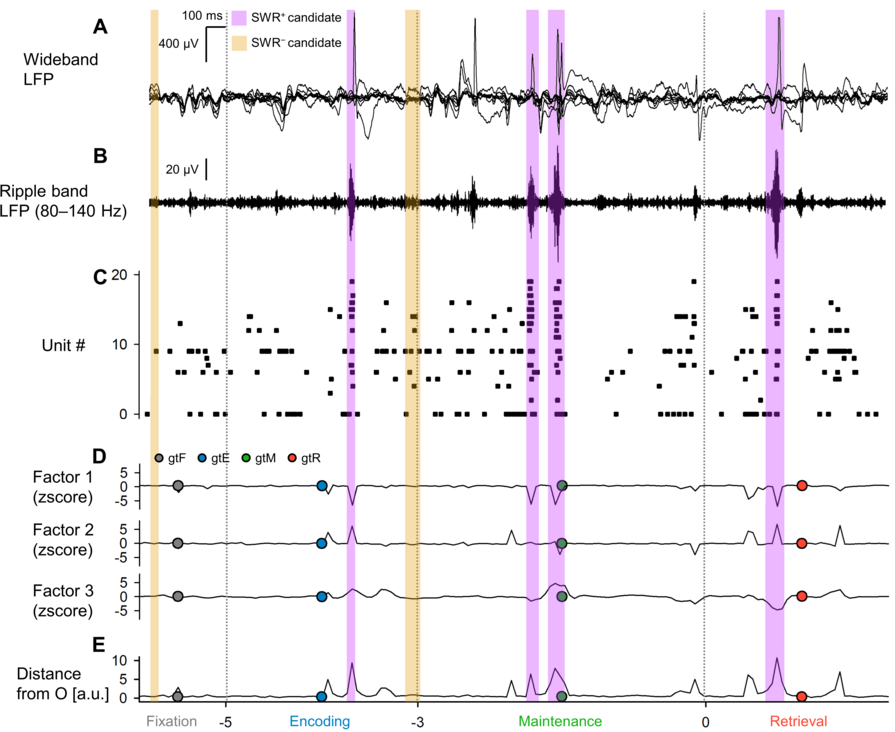
\includegraphics[width=1\textwidth]{./src/figures/.png/Figure_ID_01.png}
        	\caption{\textbf{
Local Field Potentials (LFP), Multiunit Activity, and Neural Trajectories in the Hippocampus During a Modified Sternberg Task
}
\smallskip
\\
\textbf{\textit{A.}} \DIFdelbeginFL \DIFdelFL{These traces show representative }\DIFdelendFL \DIFaddbeginFL \DIFaddFL{Representative }\DIFaddendFL wideband LFP \DIFaddbeginFL \DIFaddFL{signals for }\DIFaddendFL intracranial EEG \DIFdelbeginFL \DIFdelFL{(iEEG) signals recorded }\DIFdelendFL \DIFaddbeginFL \DIFaddFL{recording }\DIFaddendFL from the left hippocampal head. The subject performed a modified Sternberg working memory task, which includes fixation (1 s, \textit{gray}), encoding (2 s, \textit{blue}), maintenance (3 s, \textit{green}), and retrieval (2 s, \textit{red}). \textbf{\textit{B.}} \DIFdelbeginFL \DIFdelFL{We then present the }\DIFdelendFL \DIFaddbeginFL \DIFaddFL{The }\DIFaddendFL corresponding ripple band LFP traces. \DIFaddbeginFL \DIFaddFL{Note that }\textit{\DIFaddFL{purple}} \DIFaddFL{and }\textit{\DIFaddFL{yellow}} \DIFaddFL{rectangles indicating the timings for SWR$^+$ candidates and SWR$^-$ candidates (control events for SWR$^+$), respectively. }\DIFaddendFL \textbf{\textit{C.}} The raster plot depicts multiunit spikes taken from the LFP traces, sorted using a spike algorithm \cite{niediek_reliable_2016}. \textbf{\textit{D.}} \DIFdelbeginFL \DIFdelFL{Subsequently, we illustrate the neural }\DIFdelendFL \DIFaddbeginFL \DIFaddFL{Neural }\DIFaddendFL trajectories \DIFdelbeginFL \DIFdelFL{, which are }\DIFdelendFL calculated by GPFA\DIFaddbeginFL \DIFaddFL{\mbox{%DIFAUXCMD
\cite{yu_gaussian-process_2009} }\hspace{0pt}%DIFAUXCMD
}\DIFaddendFL on spike counts per unit with 50-ms bins. Each phase's geometric median is marked by the dot circles. \textbf{\textit{E.}} The \DIFdelbeginFL \DIFdelFL{trajectory's }\DIFdelendFL distance \DIFaddbeginFL \DIFaddFL{of neural trajectory }\DIFaddendFL from the origin $O$\DIFdelbeginFL \DIFdelFL{is portrayed, with }\textit{\DIFdelFL{purple}} %DIFAUXCMD
\DIFdelFL{and }\textit{\DIFdelFL{yellow}} %DIFAUXCMD
\DIFdelFL{rectangles indicating the timings for SWR$^+$ candidates and SWR$^-$ candidates (considered as controls for SWR$^+$), respectively}\DIFdelendFL .
}
% width=1\textwidth
        	\label{fig:01}
        \end{figure*}
        \clearpage
        \begin{figure*}[ht]
            \pdfbookmark[2]{ID 02}{figure_id_02}
        	\centering
            \includegraphics[width=0.5\textwidth]{./src/figures/.png/Figure_ID_02.png}
        	\caption{\textbf{
State-Dependent Trajectories of Hippocampal Neurons
}
\smallskip
\\
\textbf{\textit{A.}} Neural trajectories \DIFaddbeginFL \DIFaddFL{as a point cloud }\DIFaddendFL within the initial three-dimensional factors derived from \DIFdelbeginFL \DIFdelFL{the Gaussian Process Factor Analysis (}\DIFdelendFL GPFA \DIFdelbeginFL \DIFdelFL{) are displayed}\DIFdelendFL \DIFaddbeginFL \DIFaddFL{\mbox{%DIFAUXCMD
\cite{yu_gaussian-process_2009}}\hspace{0pt}%DIFAUXCMD
}\DIFaddendFL . The smaller dots correspond to coordinates of 50-ms neural trajectory bins, while the larger dots with \textit{black} edges \DIFdelbeginFL \DIFdelFL{signify }\DIFdelendFL \DIFaddbeginFL \DIFaddFL{show }\DIFaddendFL the geometric medians for respective \DIFdelbeginFL \DIFdelFL{stages }\DIFdelendFL \DIFaddbeginFL \DIFaddFL{phases }\DIFaddendFL in the Sternberg working memory task: fixation (\DIFaddbeginFL \DIFaddFL{$\mathrm{\lVert g_{F} \rVert}$, }\DIFaddendFL \textit{gray}), encoding (\DIFaddbeginFL \DIFaddFL{$\mathrm{\lVert g_{E} \rVert}$, }\DIFaddendFL \textit{blue}), maintenance (\DIFaddbeginFL \DIFaddFL{$\mathrm{\lVert g_{M} \rVert}$, }\DIFaddendFL \textit{green}), and retrieval (\DIFaddbeginFL \DIFaddFL{$\mathrm{\lVert g_{R} \rVert}$, }\DIFaddendFL \textit{red}). \textbf{\textit{B.}} The figure conveys the log-likelihood of the GPFA models versus the count of dimensions used to embed multiunit spikes found in the medial temporal lobe (MTL) territories. In specific, the elbow method pinpointed the optimal dimension to be three. \textbf{\textit{C.}} This panel illustrates the distance of the neural trajectories from the origin ($O$) for the hippocampus (Hipp.), entorhinal cortex (EC), and amygdala (Amy.), against the time elapsed from the probe onset. \textbf{\textit{D.}} The distance of the trajectory from $O$ within MTL regions is displayed. The hippocampus shows the farthest distance, followed by the EC and the Amygdala. \textbf{\textit{E.}} The \DIFaddbeginFL \DIFaddFL{box }\DIFaddendFL plot represents inter-phase trajectory distances within the MTL regions.
\DIFdelbeginFL \DIFdelFL{Abbreviations:
}\DIFdelendFL }
% width=0.5\textwidth
        	\label{fig:02}
        \end{figure*}
        \clearpage
        \begin{figure*}[ht]
            \pdfbookmark[2]{ID 03}{figure_id_03}
        	\centering
            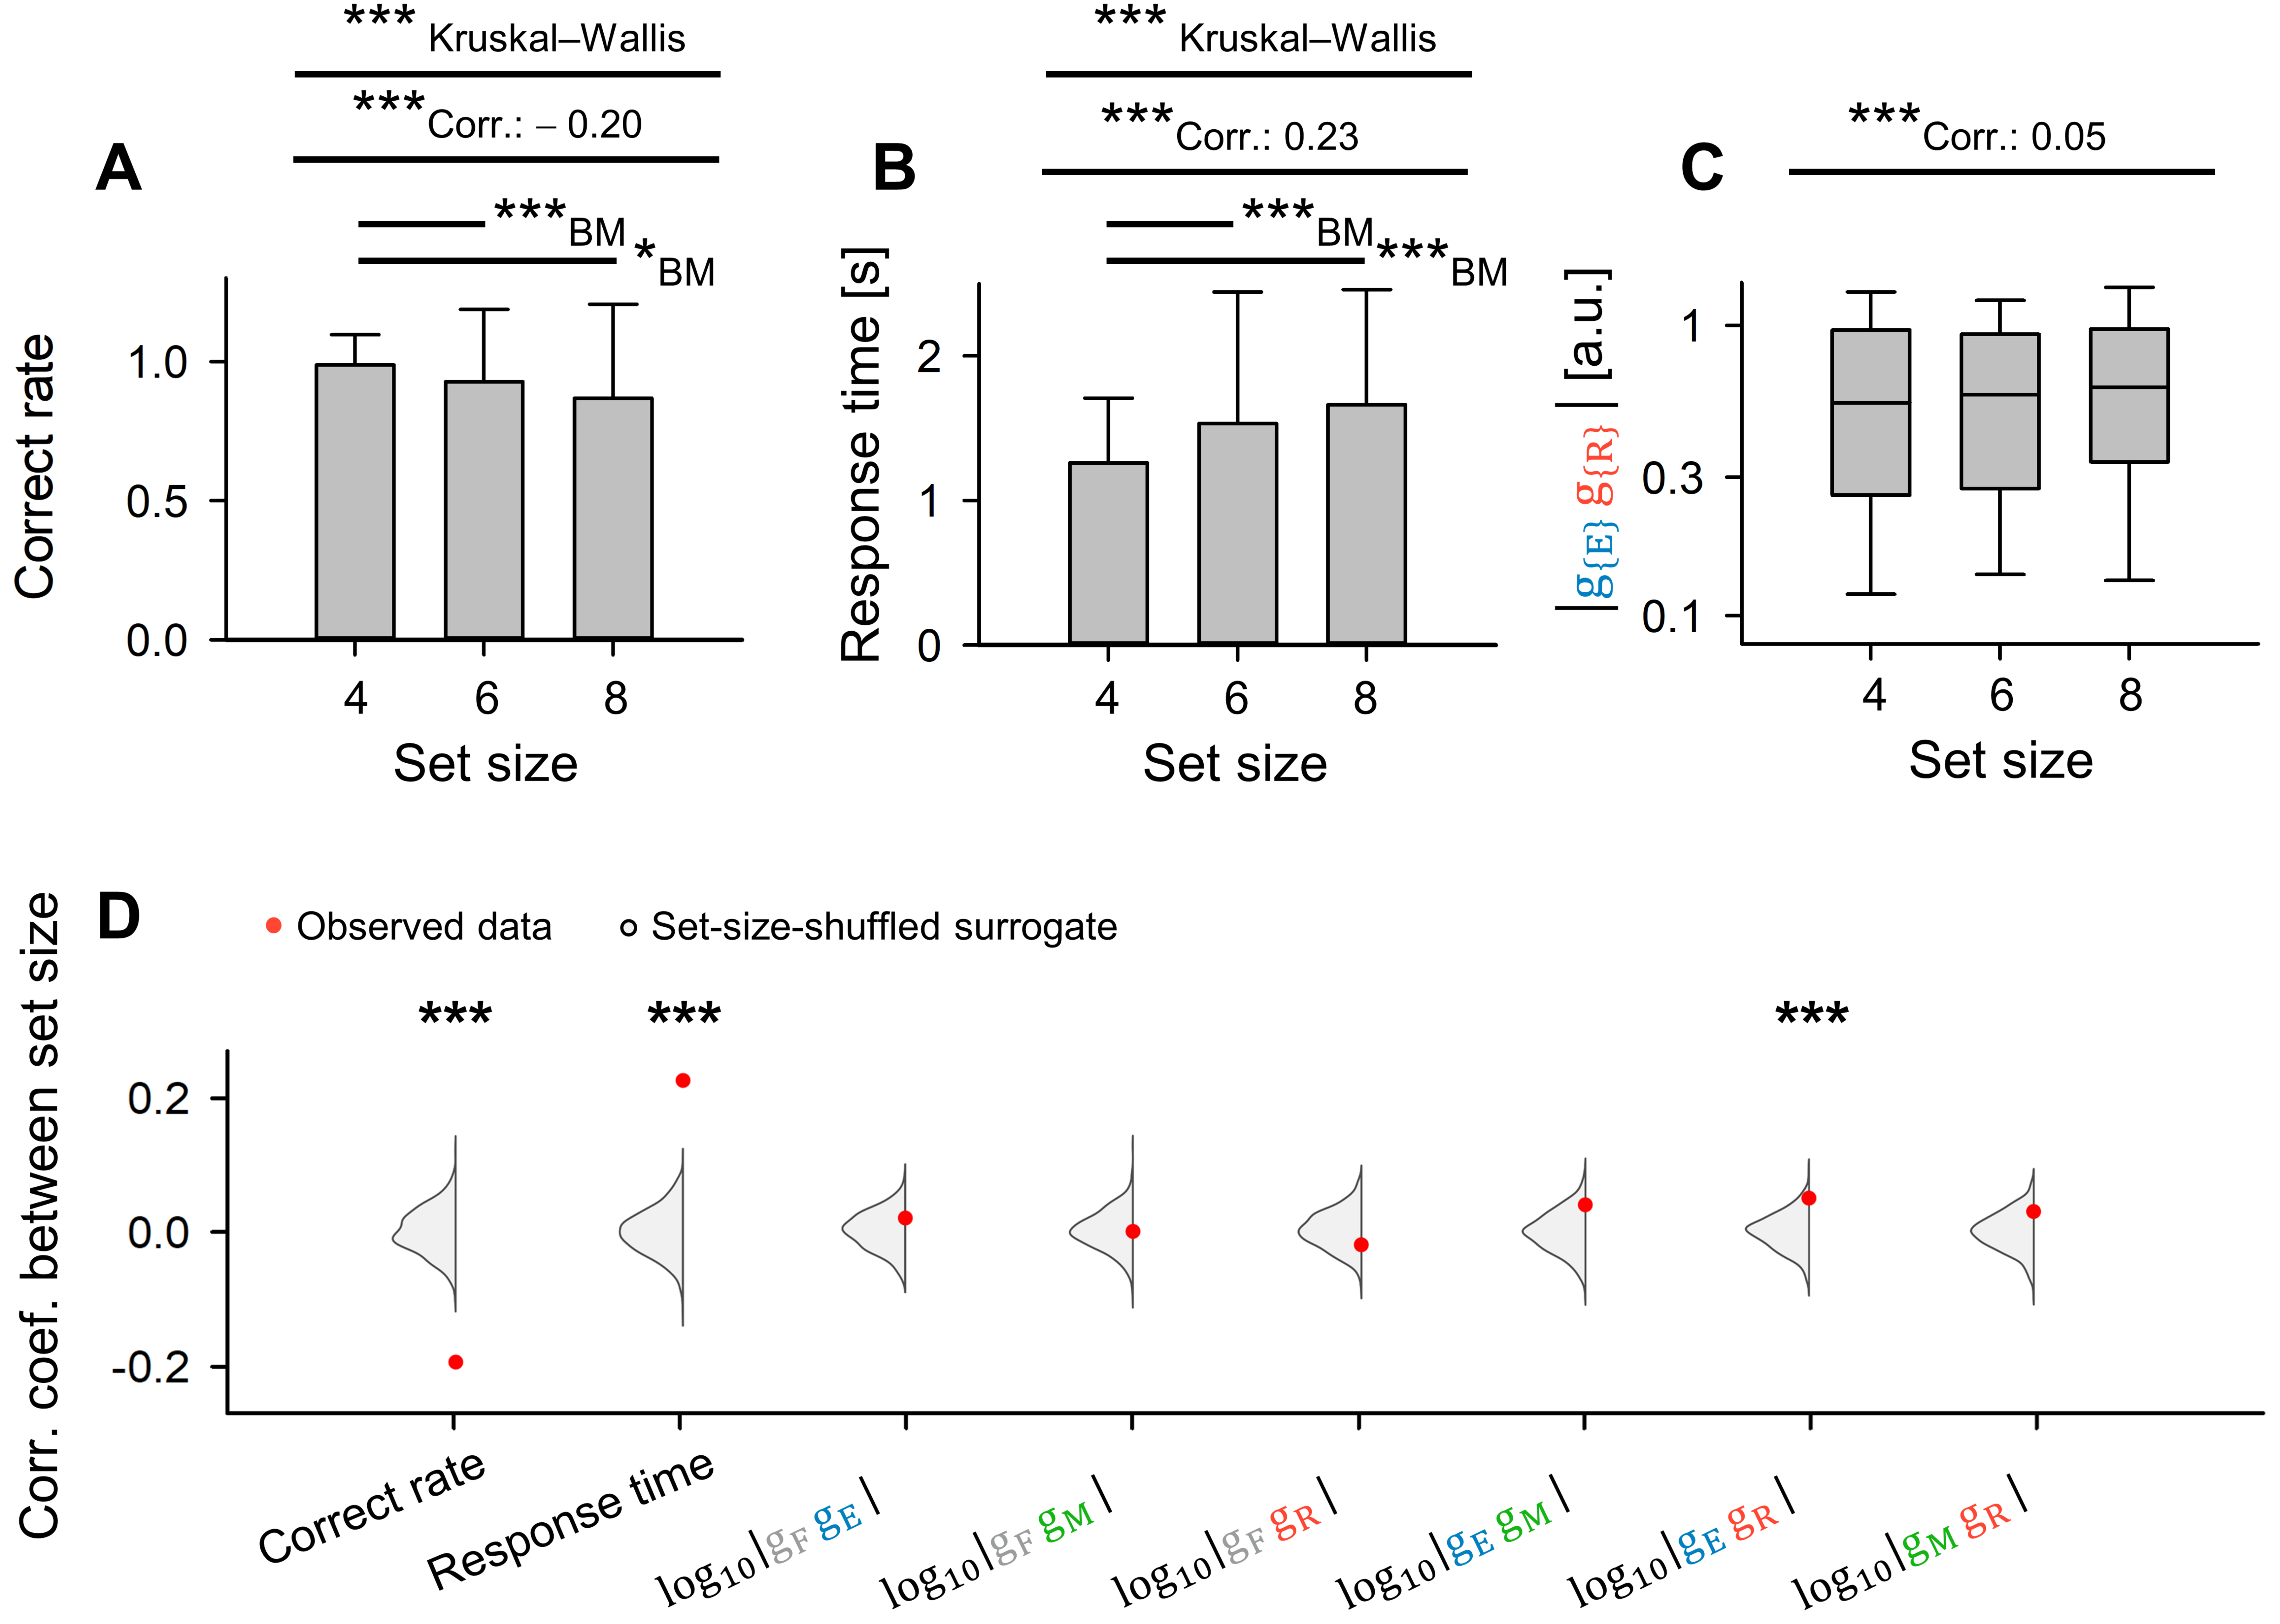
\includegraphics[width=1\textwidth]{./src/figures/.png/Figure_ID_03.png}
        	\caption{\textbf{
Dependency of Trajectory Distance on Memory Load: Encoding and Retrieval States in Hippocampus
}
\smallskip
\\
\textbf{\textit{A.}} The relationship between set size (number of letters that need to be encoded) and correct rate in the working memory task (coefficient = $-0.20$, ***\textit{p} $<$ 0.001). \textbf{\textit{B.}} The correlation between set size and response time (coefficient = 0.23, ***\textit{p} $<$ 0.001). \textbf{\textit{C.}} The impact of set size on the inter-phase distances between the encoding and retrieval phases ($\lVert \mathrm{g_{E}g_{R}} \rVert$) (correlation coefficient = 0.05\DIFaddbeginFL \DIFaddFL{, ***}\textit{\DIFaddFL{p}} \DIFaddFL{$<$ 0.001}\DIFaddendFL ). \textbf{\textit{D.}} \textit{Red} dots represent experimental observations of correlations between set size and the following parameters: correct rate, response time, $\log_{10}{\lVert \mathrm{g_{F}g_{E}} \rVert}$, $\log_{10}{\lVert \mathrm{g_{F}g_{M}} \rVert}$, $\log_{10}{\lVert \mathrm{g_{F}g_{R}} \rVert}$, $\log_{10}{\lVert \mathrm{g_{E}g_{M}} \rVert}$, $\log_{10}{\lVert \mathrm{g_{E}g_{R}} \rVert}$, and $\log_{10}{\lVert \mathrm{g_{M}g_{R}} \rVert}$. The \textit{gray} kernel density \DIFdelbeginFL \DIFdelFL{plot illustrates }\DIFdelendFL \DIFaddbeginFL \DIFaddFL{plots illustrate }\DIFaddendFL the corresponding set-size-shuffled surrogate (\textit{n} = 1,000) (***\textit{p}s $<$ 0.001).
}
% width=1\textwidth
        	\label{fig:03}
        \end{figure*}
        \clearpage
        \begin{figure*}[ht]
            \pdfbookmark[2]{ID 04}{figure_id_04}
        	\centering
            \includegraphics[width=1\textwidth]{./src/figures/.png/Figure_ID_04.png}
        	\caption{\textbf{
Detection of SWRs in Presumptive CA1 Regions
}
\smallskip
\\
\textbf{\textit{A.}} Two-dimensional UMAP \DIFdelbeginFL \DIFdelFL{(Uniform Manifold Approximation and Projection) }\DIFdelendFL \cite{mcinnes_umap_2018} projection of multiunit spikes during SWR$^+$ candidates (\textit{purple}) and SWR$^-$ candidates (\textit{yellow}). \textbf{\textit{B.}} Cumulative density plot \DIFdelbeginFL \DIFdelFL{shows }\DIFdelendFL \DIFaddbeginFL \DIFaddFL{showing }\DIFaddendFL silhouette scores, indicative of UMAP clustering quality \DIFdelbeginFL \DIFdelFL{, for hippocampal regions }\DIFdelendFL (see Table~\ref{tab:02}\DIFdelbeginFL \DIFdelFL{for reference}\DIFdelendFL ). Note that hippocampal regions with silhouette scores greater than 0.60 (equivalent to the $75^{th}$ percentile) were \DIFdelbeginFL \DIFdelFL{identified }\DIFdelendFL \DIFaddbeginFL \DIFaddFL{defined }\DIFaddendFL as \DIFdelbeginFL \DIFdelFL{possible }\DIFdelendFL \DIFaddbeginFL \DIFaddFL{putative }\DIFaddendFL CA1 regions. SWR$^+$ and SWR$^-$ candidates recorded from these \DIFdelbeginFL \DIFdelFL{speculative }\DIFdelendFL \DIFaddbeginFL \DIFaddFL{putative }\DIFaddendFL CA1 regions were respectively classified as SWR$^+$ and SWR$^-$ (\textit{n}s = 1,170). \textbf{\textit{C.}} The identical distributions of durations are presented for SWR$^+$ (\textit{purple}) and SWR$^-$ (\textit{yellow}), owing to their definitions (93.0 [65.4] ms, median [IQR]). \textbf{\textit{D.}} SWR incidence for both SWR$^+$ (\textit{purple}) and SWR$^-$ (\textit{yellow}) obtained relative to the probe's timing is illustrated as a mean \textpm 95\% confidence interval. However, as the intervals may not be visible due to their narrow \DIFdelbeginFL \DIFdelFL{range}\DIFdelendFL \DIFaddbeginFL \DIFaddFL{ranges}\DIFaddendFL , note that a significant increase in SWR incidence was detected during the initial 400 ms of the retrieval phase (0.421 [Hz], *\textit{p} $<$ 0.05, bootstrap test). \textbf{\textit{E.}} The distributions of ripple band peak amplitudes for SWR$^-$ (\textit{yellow}; 2.37 [0.33] SD of baseline, median [IQR]) and SWR$^+$ (\textit{purple}; 3.05 [0.85] SD of baseline, median [IQR]) are delineated (***\textit{p} $<$ 0.001, the Brunner--Munzel test).
}
% width=1\textwidth
        	\label{fig:04}
        \end{figure*}
        \clearpage
        \begin{figure*}[ht]
            \pdfbookmark[2]{ID 05}{figure_id_05}
        	\centering
            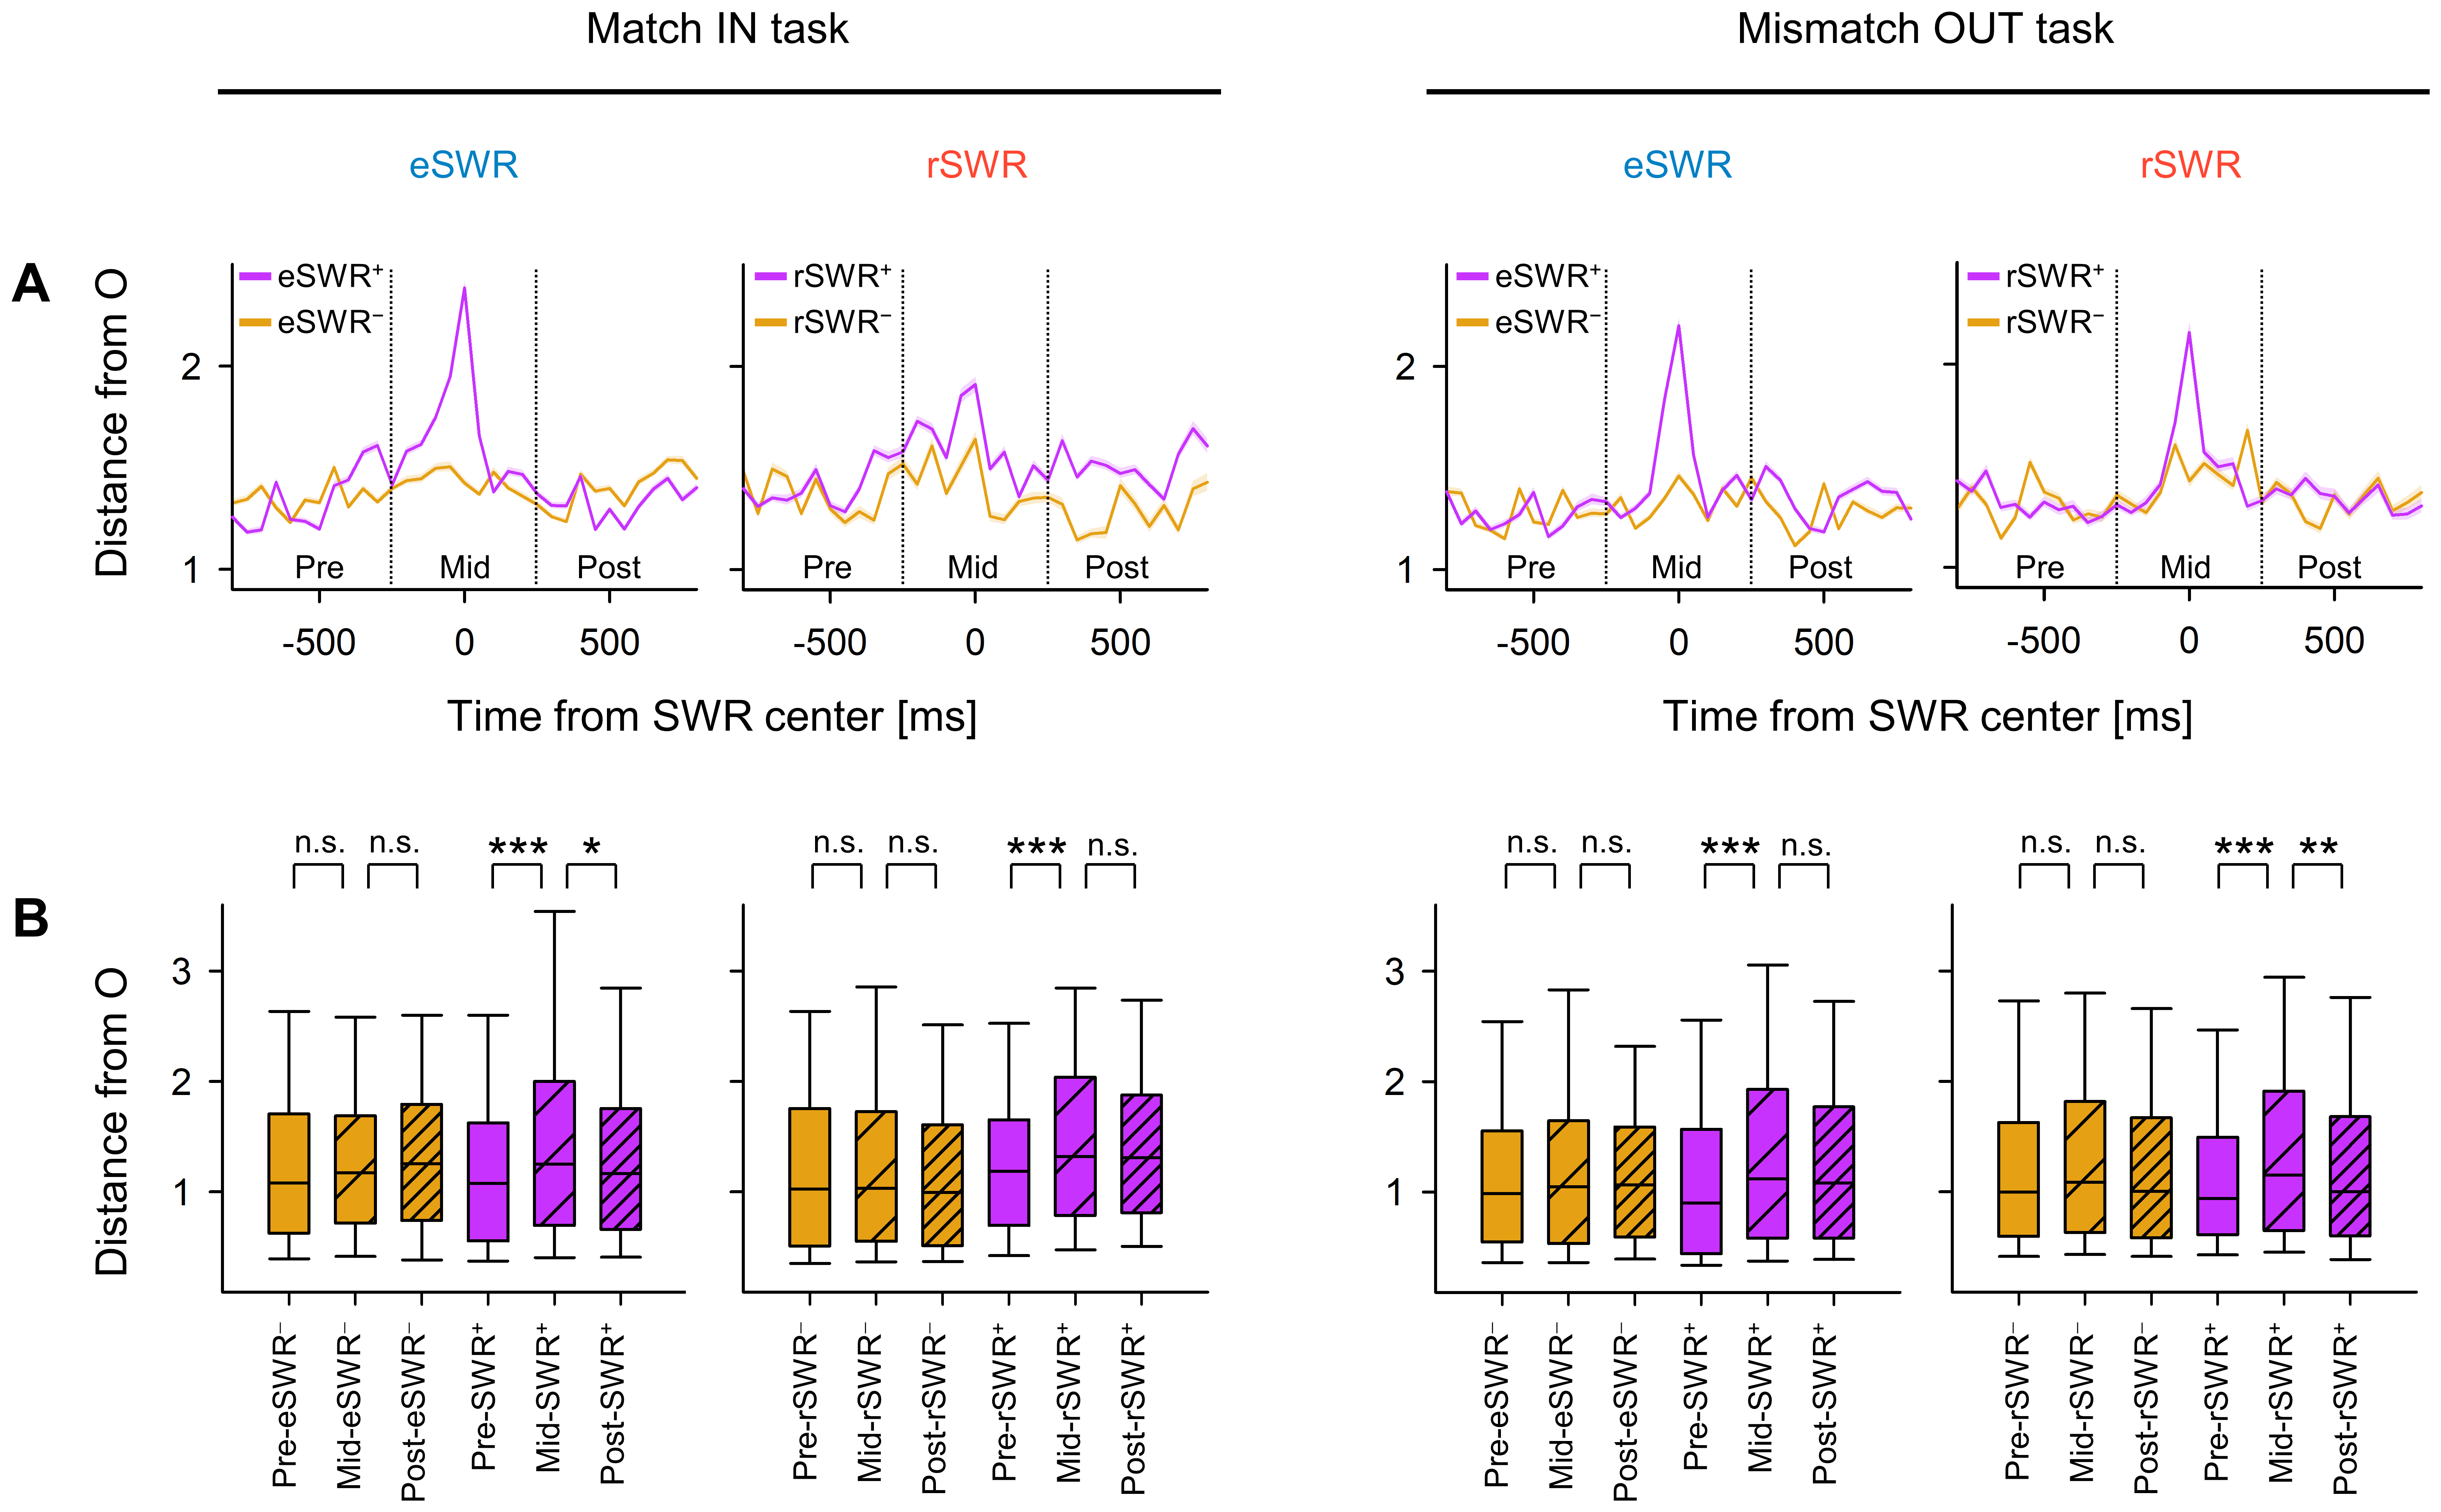
\includegraphics[width=1\textwidth]{./src/figures/.png/Figure_ID_05.png}
        	\caption{\textbf{
Transient Alterations in Neural Trajectory During SWR Events
}
\smallskip
\\
\textbf{\textit{A.}} Displayed is the distance from origin ($O$) of the peri-sharp-wave-ripple trajectory (mean \textpm 95\% confidence interval). The intervals may not be apparent due to their \DIFdelbeginFL \DIFdelFL{slender }\DIFdelendFL \DIFaddbeginFL \DIFaddFL{narrow }\DIFaddendFL ranges. \textbf{\textit{B.}} Shown is the distance from the origin ($O$) during pre-, mid-, and post-SWR periods (*\textit{p} $<$ 0.05, **\textit{p} $<$ 0.01, ***\textit{p} $<$ 0.001; \DIFdelbeginFL \DIFdelFL{assessed using }\DIFdelendFL the Brunner--Munzel test). Abbreviations: SWR, sharp-wave ripple events; eSWR, SWR during the encoding phase; rSWR, SWR while in the retrieval phase; SWR$^+$, positive SWR event; SWR$^-$, control events for SWR$^+$; pre-, mid-, or post-SWR denote the time intervals from $-800$ to $-250$ ms, from $-250$ to $+250$ ms, or from $+250$ to $+800$ ms, all relative to the center of the SWR.
}
% width=1\textwidth
        	\label{fig:05}
        \end{figure*}
        \clearpage
        \begin{figure*}[ht]
            \pdfbookmark[2]{ID 06}{figure_id_06}
        	\centering
            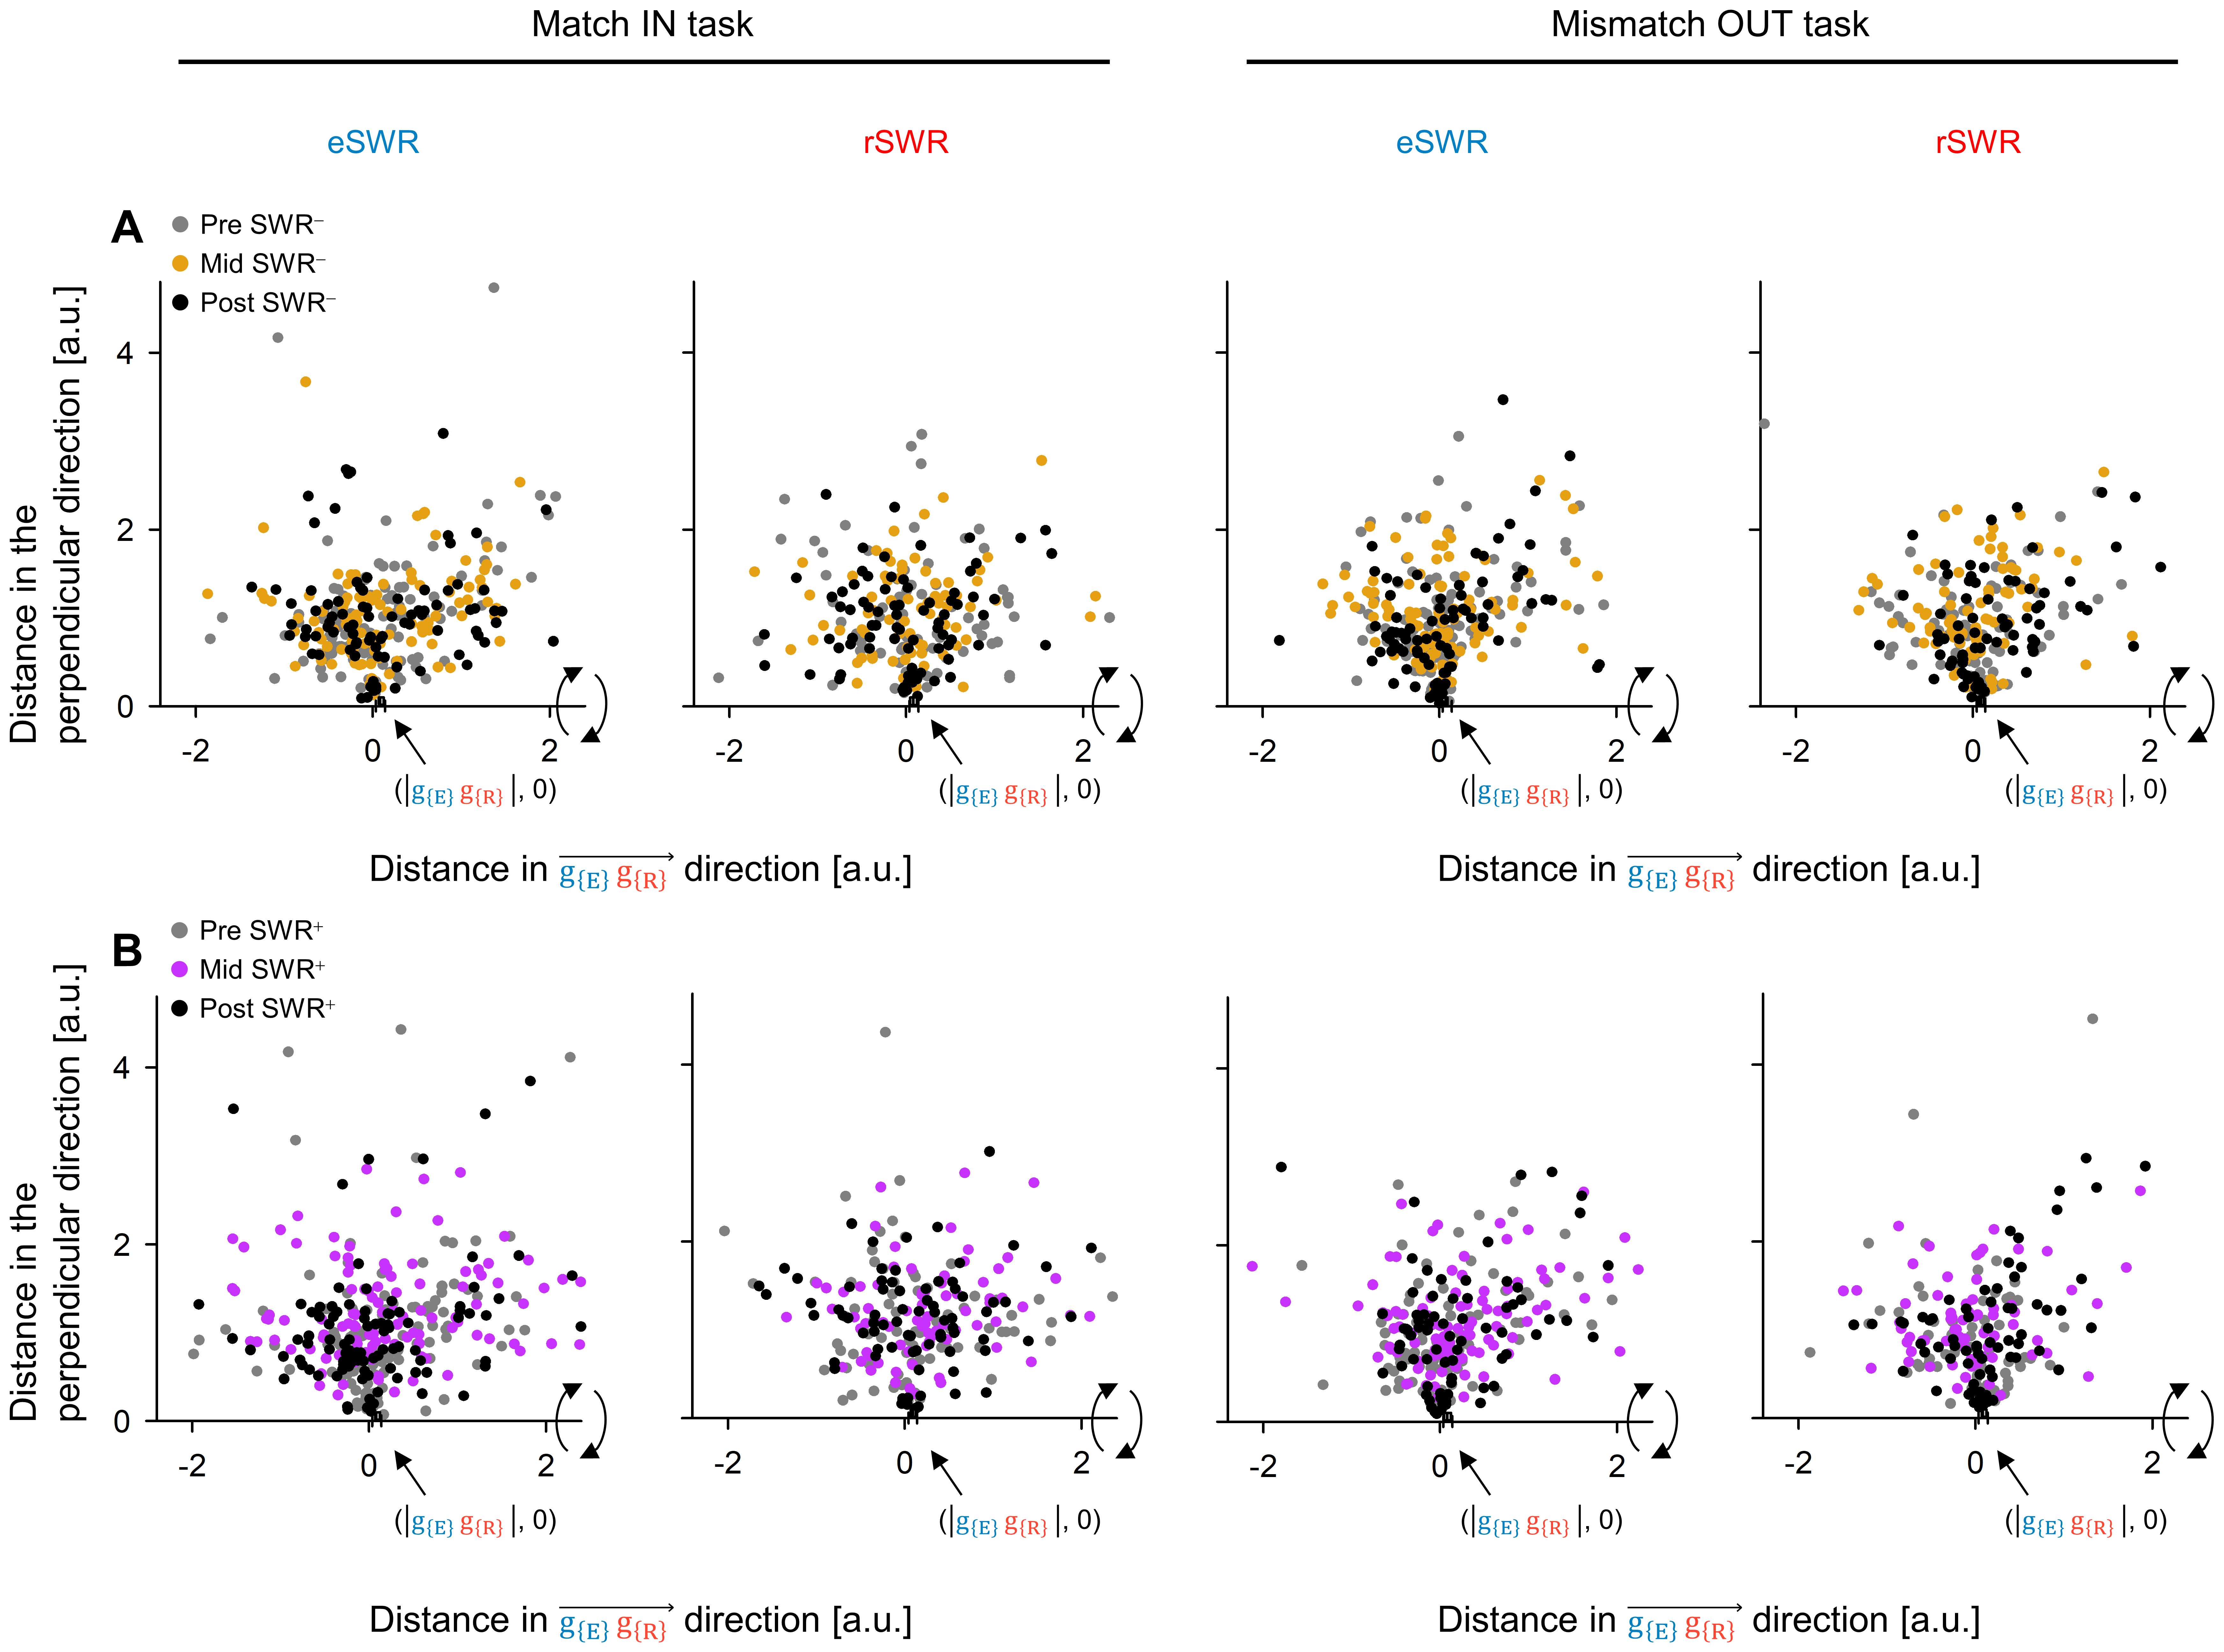
\includegraphics[width=1\textwidth]{./src/figures/.png/Figure_ID_06.png}
        	\caption{\textbf{
Visualization of Neural Trajectories during SWR in Two-Dimensional Spaces}
\smallskip
\\
The panels display hippocampal neural trajectories during SWR as projected onto two-dimensional spaces. \textbf{\textit{A.}} \DIFdelbeginFL \DIFdelFL{Indicates hippocampal }\DIFdelendFL \DIFaddbeginFL \DIFaddFL{Hippocampal }\DIFaddendFL neural trajectories \DIFaddbeginFL \DIFaddFL{as point clouds during }\DIFaddendFL pre-SWR$^-$ (\textit{gray}), mid-SWR$^-$ (\textit{yellow}), and post-SWR$^-$ (\textit{black}). \textbf{\textit{B.}} Represents the equivalents for SWR$^+$ as opposed to SWR$^-$. The \DIFdelbeginFL \DIFdelFL{$\lVert \mathrm{g_{E}g_{R}} \rVert$ varied among sessions. The }\DIFdelendFL projection was applied in the following manner: First, a linear transformation positioned $\mathrm{g_{E}}$ at the origin $O$ (0,0), and $\mathrm{g_{R}}$ at ($\lVert \mathrm{g_{E}g_{R}} \rVert$, 0). The point cloud was then rotated around the $\mathrm{g_{E}g_{R}}$ axis (equivalent to the x axis) for fitting into two-dimensional spaces. Therefore, within these two-dimensional spaces, both the distances from $O$ and the angles \DIFdelbeginFL \DIFdelFL{preserved the original makeup of }\DIFdelendFL \DIFaddbeginFL \DIFaddFL{for }\DIFaddendFL the $\mathrm{g_{E}g_{R}}$ axis \DIFdelbeginFL \DIFdelFL{from }\DIFdelendFL \DIFaddbeginFL \DIFaddFL{are preserved }\DIFaddendFL the original \DIFdelbeginFL \DIFdelFL{three-dimensional }\DIFdelendFL \DIFaddbeginFL \DIFaddFL{three dimensional }\DIFaddendFL spaces \DIFaddbeginFL \DIFaddFL{in GPFA}\DIFaddendFL . Abbreviations: SWR signifies sharp-wave ripple events; eSWR denotes SWR during the encoding phase; rSWR indicates SWR during the retrieval phase; SWR$^+$, marks an SWR event; SWR$^-$ refers to control events for SWR$^+$; pre-SWR, mid-SWR, or post-SWR, reference the time intervals from $-800$ to $-250$ ms, from $-250$ to $+250$ ms, or from $+250$ to $+800$ ms from the center of SWR.
}
% width=1\textwidth
        	\label{fig:06}
        \end{figure*}
        \clearpage
        \begin{figure*}[ht]
            \pdfbookmark[2]{ID 07}{figure_id_07}
        	\centering
            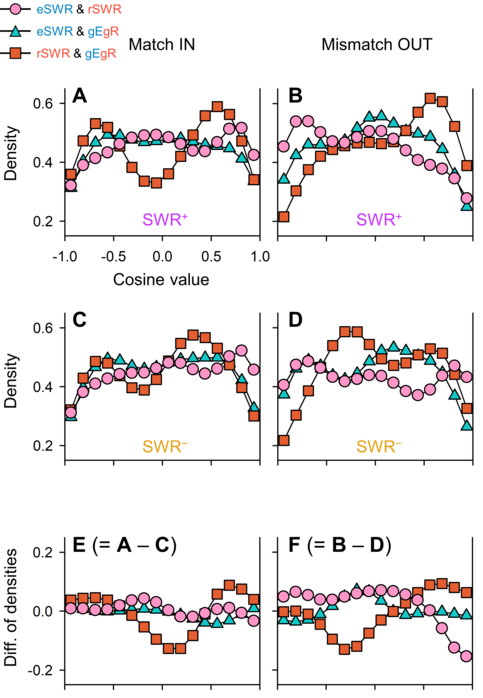
\includegraphics[width=0.5\textwidth]{./src/figures/.png/Figure_ID_07.png}
        	\caption{\textbf{
Directions of Neural Trajectories during SWRs Based on Encoding and Retrieval States
}
\smallskip
\\
\textbf{\textit{A--B}} Kernel density estimation \DIFdelbeginFL \DIFdelFL{(KDE) }\DIFdelendFL distributions of $\protect\overrightarrow{{\mathrm{eSWR^+}}} \cdot \protect\overrightarrow{{\mathrm{rSWR^+}}}$ (\textit{pink circles}), $\protect\overrightarrow{{\mathrm{eSWR^+}}} \cdot \protect\overrightarrow{{\mathrm{g_{E}g_{R}}}}$ (\textit{blue triangles}), and $\protect\overrightarrow{{\mathrm{rSWR^+}}} \cdot \protect\overrightarrow{{\mathrm{g_{E}g_{R}}}}$ (\textit{red rectangles}) in Match In (\textit{A}) and Mismatch OUT tasks (\textit{B}). \textbf{\textit{C--D}} Present the corresponding distributions of $\mathrm{SWR^-}$ instead of those of $\mathrm{SWR^+}$ in \textit{A} and \textit{B}. \textbf{\textit{E--F}} Depict the differences in the distributions of $\mathrm{SWR^+}$ and $\mathrm{SWR^-}$, illuminating the SWR components (\textit{E} = \textit{C} $-$ \textit{A} \DIFdelbeginFL \DIFdelFL{; }\DIFdelendFL \DIFaddbeginFL \DIFaddFL{\& }\DIFaddendFL \textit{F} = \textit{D} $-$ \textit{B}). Note the biphasic distributions of $\protect\overrightarrow{{\mathrm{rSWR^-}}} \cdot \protect\overrightarrow{{\mathrm{g_{E}g_{R}}}}$, suggesting fluctuations between the encoding and retrieval states during the Sternberg task. Moreover, inverse directionality between $\protect\overrightarrow{{\mathrm{eSWR^+}}}$ and $\protect\overrightarrow{{\mathrm{rSWR^+}}}$ was observed (\textit{pink circles}) \DIFdelbeginFL \DIFdelFL{in the Mismatch OUT task, but }\DIFdelendFL not in the Match IN task \DIFdelbeginFL \textbf{\textit{\DIFdelFL{E--F}}%DIFAUXCMD
}%DIFAUXCMD
\DIFdelendFL \DIFaddbeginFL \textbf{\textit{\DIFaddFL{E}}}\DIFaddendFL )\DIFdelbeginFL \DIFdelFL{. }\DIFdelendFL \DIFaddbeginFL \DIFaddFL{) but in Mismatch OUT task }\textbf{\textit{\DIFaddFL{F}}}\DIFaddFL{), }\DIFaddendFL Finally, shifts from the retrieval to encoding states \DIFdelbeginFL \DIFdelFL{were evident }\DIFdelendFL \DIFaddbeginFL \DIFaddFL{are acknowledged }\DIFaddendFL in the SWR components in both \DIFdelbeginFL \DIFdelFL{the }\DIFdelendFL Match IN and Mismatch OUT tasks (\textit{red rectangles} in \DIFdelbeginFL \textit{\DIFdelFL{E}} %DIFAUXCMD
\DIFdelFL{and }\textit{\DIFdelFL{F}}%DIFAUXCMD
\DIFdelendFL \DIFaddbeginFL \textit{\DIFaddFL{E--F}}\DIFaddendFL ).
}
% width=0.5\textwidth
        	\label{fig:07}
        \end{figure*}

%%%%%%%%%%%%%%%%%%%%%%%%%%%%%%%%%%%%%%%%%%%%%%%%%%%%%%%%%%%%%%%%%%%%%%%%%%%%%%%%
%% END
%%%%%%%%%%%%%%%%%%%%%%%%%%%%%%%%%%%%%%%%%%%%%%%%%%%%%%%%%%%%%%%%%%%%%%%%%%%%%%%%

\end{document}
